\chapterimage{anexos/html/imagenes/cover}
\chapterimagedescription{Imágen de un diseñador web pensando en código}
\chapterimageauthor{Diseño de Mudassar Iqbal con retoques propios}

\chapter{HTML}
\label{HTML}

\textbf{HyperText Markup Language (HTML)} es un lenguaje de marcado que sirve
para describir páginas web, por lo que se ha transformado en el lenguaje de
marcado más extendido del mundo.

HTML es un lenguaje basado en XML, por lo que su principio fundamental son las
etiquetas, que actúan de marcas para indicar distintos tipos de contenidos en la
página web que describen.

Un archivo de HTML es simplemente un archivo de texto, que en general se identifican
con la extensión \textbf{.html}, y que puede editarse con cualquier editor de
texto. Para visualizar el contenido como un sitio web, se debe utilizar un
programa visualizador especial, que en general se conoce como \textbf{browser} o
\textbf{navegador web}.

\section{Browsers}

El browser tiene una doble funcionalidad, por un lado, permite conectarse a
dispositivos remotos, los cuales se identifican con una URL específica, y descargar
de este uno o más archivos. Por otro lado permite visualizar los archivos HTML,
interpretando su contenidos y dando una muestra visual de los contenidos (Esto
incluye la interpretación de CSS y de JavaScript). Cuando uno coloca una URL
como ``\href{http://google.com}'', el browser ingresa a la máquina identificada
como ``google.com'' y descarga por defecto el archivo ``index.html'' del mismo.
Otras URLs, como ``\href{http://google.com/archivo.html}'' descargan el archivo
específico ``archivo.html''.

Existen muchos browsers en el mercado, algunos privativos, otros libres. Entre
los más destacados están:
\begin{itemize}
    \item Internet Explorer
    \item Edge
    \item Google Chrome
    \item Mozilla Firefox
    \item Opera
\end{itemize}

\section{W3C y estándares de la web}

A diferencia de otros lenguajes, HTML se encuentra claramente especificado en lo
que se conoce como el estándar HTML, el cual está definido por el \textbf{World
Wide Web Consortium (W3C)}, una organización encargada de definir estándares para la web,
y promover su correcto uso.

\image{anexos/html/imagenes/browsers.png}
{Logos de diferentes browsers. Existe una amplia diversidad, con navegadores que
se enfocan en mercados sumamente específicos.}
{Logos del proyecto \href{github.com/alrra/browser-logos}{github.com/alrra/browser-logos}.}

Cabe destacar que HTML define una estructura para el contenido, y son los navegadores
los que determinan de que forma mostrar dicho contenido (el estilo). Si se desea
especificar estilos más avanzados, debe recurrirse al uso de otro lenguaje de la
web, conocido como ``Hojas de Estilo en Cascada'', o en inglés \textbf{Cascade
Style Sheets (CSS)}. Este lenguaje complementa a HTML, permitiendo definir cosas
como los colores de texto, tamaños de fuentes, ubicación de imágenes, colores de
fondo, distribución de contenidos en la página, entre una gran serie de otros
elementos. CSS también está especificado por la W3C.

Finalmente, si lo que se desea es lograr una interactividad en el sitio (por ejemplo,
que se muestre cierto contenido cuando el usuario selecciona una opción, o cuando
presiona un botón), se debe recurrir a un lenguaje de programación conocido como
\textbf{JavaScript} (o \textbf{ECMAScript}), el cual permite manipular las etiquetas
del documento HTML, agregando o quitando contenido, atributos, e incluso nuevas
etiquetas en cualquier lugar del documento. JavaScript también está definido por
la W3C, complementando así los otros lenguajes.

La W3C también define otros estándares que permiten la definición de imágenes
vectoriales para la web, o formatos de transmisión de datos entre equipos, entre
otra serie de cosas.

A lo largo del tiempo se han definido varias versiones de HTML, siendo las primeras
bastante primitivas, permitiendo poca interacción con el usuario, mientras que
actualmente se puede definir aplicaciones enteras usando HTML, CSS y JavaScript.
La versión actual de HTML es la versión 5, y es una versión ``viva'', es decir,
no hay una versión 5 final, sino que el estándar se va actualizando a medida que
surge la necesidad de utilizar nuevas etiquetas. Así, algunas etiquetas clásicas
desaparecen, y otras nuevas aparecen. Junto con HTML5 aparecen nuevos estándares
para CSS (CSS 3, también una versión ``viva''), y JavaScript (En versiones cada
vez más modernas adhiriendo al estándar ECMAScript que publica una nueva versión
cada año).

Por ser tan longevo, y por las cualidades de ser un lenguaje vivo, la documentación
que uno puede encontrar en Internet sobre HTML puede estar desactualizada y haberse
vuelto obsoleta. A esto se debe sumar el hecho de que mucha gente aprende por su
cuenta, y luego hace público su conocimiento, el cuál no siempre es correcto. Por
eso es importante para los desarrolladores web seguir los estándares de la W3C y
asegurarse de que su código siga dichos estándares.

¿Qué ocurre si nuestro código no sigue el estándar? En principio, nada.
Cualquier ``buen browser'' (entiéndase casi todos los navegadores web modernos,
a excepción de Internet Explorer) garantiza que los códigos que siguen el
estándar de la W3C se verán correctamente. Sin embargo, cada uno tiene su
propia implementación, y su propia idea de ``que hacer'' ante código que no
sigue la norma. Así, código que funciona en Google Chrome puede no verse bien
en Firefox o en Internet Explorer. 

Si nos encontramos realizando un sitio que va a ser utilizado por el público en
general, debemos seguir necesariamente el estándar, pues no podemos garantizar
cual es el navegador web que va a utilizar la persona que ingrese. Internet
Explorer, por gozar de una situación monopólica en la mayoría de los equipos
domésticos, pudo no seguir los estándares. Esto hacía que cualquier desarrollador
que hiciera una página, debía realizar dos versiones de la misma, una para
Internet Explorer, y otra para el resto de los navegadores. La situación se
mantuvo hasta la salida de Edge por parte de Microsoft, reemplazando a Internet
Explorer, forzada por las decisiones de múltiples empresas y desarrolladores de
dejar de dar soporte a Internet Explorer.

\section{Sistema de etiquetas como marcas}

En los lenguajes basados a etiquetas, la etiqueta es el elemento fundamental
que permite marcar una porción de texto, y es, en si mismo, un elemento que
puede ser marcado por otras etiquetas.

Toda etiqueta está dada por una marca que comienza por el signo ``<'' (menor),
se sigue de un \textbf{nombre}, y cierra con el signo ``>'' (mayor). El nombre
de la etiqueta consiste en una única palabra, que puede contener letras, números,
guiones bajos o guiones medios (no puede tener espacios).

Además, la mayoría de las etiquetas consisten en dos marcas, una como la
mencionada anteriormente, conocida como marca de ``\textbf{apertura}'', y otra
que es conocida como marca de ``\textbf{cierre}'', y que a diferencia de la
anteriores utiliza ``</'' (menor seguido de barra) para el comienzo de la marca.

Así, la siguiente es la marca  de apertura:
\begin{lstlisting}[language=XHTML]
<nombre_de_etiqueta>
\end{lstlisting}

Y la siguiente una etiqueta de cierre:
\begin{lstlisting}[language=XHTML]
</nombre_de_etiqueta>
\end{lstlisting}

El nombre de la etiqueta debe ser el mismo tanto en la marca de apertura
como en la de cierre. La etiqueta marca el texto que se encuentra entre
la marca de apertura y la de cierre, llamado ``\textbf{contenido}'' de la etiqueta.

\begin{lstlisting}[language=XHTML]
<nombre_etiqueta> Contenido </nombre_etiqueta>
\end{lstlisting}

El contenido de una etiqueta pueden ser otras etiquetas:
\begin{lstlisting}[language=XHTML]
<etiqueta1>
    <etiqueta2>
        Contenido de la etiqueta
    </etiqueta2>
</etiqueta1>
\end{lstlisting}

También puede darse el caso de que se requiera información adicional para marcar
un texto que el solo nombre de la etiqueta. Esa información adicional puede
ser brindada a la etiqueta mediante un ``\textbf{atributo}''. Un atributo consiste en un
par de elementos, conocidos como ``\textbf{clave}'' (el nombre del atributo)
y ``\textbf{valor}'' (el valor del atributo). Estos se colocan únicamente en la
etiqueta de apertura, separando la clave del valor mediante un signo igual (=),
y donde el valor siempre debe escribirse entre comillas.

\begin{lstlisting}[language=XHTML]
<nombre_de_etiqueta atributo="valor">
\end{lstlisting}

En una misma etiqueta pueden colocarse tantos atributos como se desee, separando
cada atributo del otro con un espacio. Note como el primer atributo también
se separa del nombre de la etiqueta mediante un espacio.

\begin{lstlisting}[language=XHTML]
<nombre attr1="val1" attr2="val2">
\end{lstlisting}

Finalmente, en ocasiones es necesario agregar contenido que sea ignorado por
el visualizador. Este contenido sirve para que el mismo autor del código pueda
estructurar sus ideas, o dejar mensajes a otros posibles lectores del código
fuente, y se conocen como ``\textbf{comentarios}''.

Un comentario comienza cuando se encuentran los signos ``<!--'' y termina cuando 
se encuentran los signos ``-->''. Un comentario puede abarcar varias etiquetas,
e incluso varias líneas de texto.

\begin{lstlisting}[language=XHTML]
<!--
    Esto es un comentario,
    puede ponerse lo que se desee aquí, 
    incluso etiquetas como <hola> o </hola>
    y serán ignoradas
-->
\end{lstlisting}

Además, vale aclarar que en HTML, así como en otros lenguajes de etiquetas, un
espacio, múltiples espacios, una o más tabulaciones, o incluso uno o más saltos
de línea son equivalentes a un único espacio. Así, estas cuatro etiquetas son
exactamente equivalentes:

\begin{lstlisting}[language=XHTML]
<etiqueta attr1="val1" attr2="val2">
<etiqueta       attr1="val1"       attr2="val2">
<etiqueta attr1="val1"
          attr2="val2">
<etiqueta
    attr1="val1"
    attr2="val2"
>
\end{lstlisting}

Note como el signo ``>'' de cierre de la marca, puede también estar en otra línea.
También vale para el de apertura.

Por último, considere el siguiente código:
\begin{lstlisting}[language=XHTML]
<etiqueta1><etiqueta2>Contenido de la etiqueta
</etiqueta2><etiqueta2 attr="val1"><etiqueta3>Contenido de la etiqueta 3
</etiqueta3>
</etiqueta2></etiqueta1>
\end{lstlisting}

Observe como se vuelve complicado identificar que etiqueta contiene a que otra,
y qué marca tiene cada uno. Considere ahora la siguiente versión con el mismo
código, pero estructurado de una forma diferente:

\begin{lstlisting}[language=XHTML]
<etiqueta1>
    <etiqueta2>
        Contenido de la etiqueta
    </etiqueta2>
    <etiqueta2 attr="val1">
        <etiqueta3>
            Contenido de la etiqueta 3
        </etiqueta3>
    </etiqueta2>
</etiqueta1>
\end{lstlisting}

Observe como esta forma de estructurar el contenido facilita su lectura y
su entendimiento. Esto se conoce en programación como ``\textbf{indentación del
código}'', es decir, tabular y estructurar el código de forma tal que sea fácil
identificar las partes del mismo. La palabra ``indentación'' viene de la palabra
inglesa ``indent', y su equivalente en español sería ``tabulado''. Es deseable
que todo el código se encuentre correctamente indentado. En los lenguajes de
etiquetas, cada marca de cierre debería colocarse a la misma altura horizontal
que su marca de cierre. Luego, el contenido dentro de una etiqueta se debe colocar
en una nueva línea y siempre tabulado dos o cuatro espacios (un ancho de tabulación)
más a la derecha que la etiqueta que lo contiene.

\section{Etiquetas básicas de HTML}

HTML, como lenguaje de etiquetas, sigue la misma estructura mencionada en la
sección anterior, pero el conjunto de etiquetas que pueden utilizarse y la
forma en la que deben estructurarse las mismas. También, el efecto que produce
cada etiqueta al ser visualizada está definido en la especificación del lenguaje.

Existen etiquetas para una gran cantidad de elementos, y este apunte no pretende
ser una guía comprensiva de los mismos, así como tampoco estar necesariamente
actualizado. Por esto se recomienda tener a mano los siguientes enlaces para
aprender sobre nuevas etiquetas o validar la información sobre las aquí expuestas.

\begin{itemize}
    \item \href{https://developer.mozilla.org/es/}{https://developer.mozilla.org/es/}
    \item \href{https://www.w3schools.com}{https://www.w3schools.com}
\end{itemize}


\subsection*{Párrafos y énfasis}

La etiqueta más sencilla que permite definir un párrafo de texto es
``\textbf{<p>}''. Dentro de ``<p>' solamente debería haber texto, el cuál puede
o no estar enfatizado en algún lugar.

\begin{lstlisting}[language=XHTML]
<p>
    El texto aquí presente compone un párrafo, el
    cuál empieza en la marca de apertura y termina
    en la marca de cierre.
</p>
<p>
    Al abrir una nueva etiqueta, el contenido de
    esta se encuentra en otro párrafo.
</p>
\end{lstlisting}

Cada párrafo se encuentra separado del siguiente por un pequeño espacio, cuyo
tamaño inicial es delimitado por el browser. Si se requiere una mayor distancia
entre un párrafo y el siguiente (u otros elementos que lo rodean) se debe utilizar
CSS.

También se puede dar énfasis a palabras o frases enteras dentro de un párrafo.
Para ello existen dos etiquetas, ``\textbf{<em>}'' que da un énfasis simple, y
``\textbf{<strong>}'', el cuál da un énfasis doble. El énfasis simple suele ser
mostrado por defecto en itálica, mientras que el doble suele ser mostrado en
negrita. Nuevamente, este comportamiento puede variarse con CSS.

\begin{lstlisting}[language=XHTML]
<p>
    En este párrafo <em>éste texto está siendo
    enfatizado</em>, y el que sigue también,
    <strong>pero con un énfasis aún mayor</strong>
</p>
\end{lstlisting}

Si bien es posible colocar una etiqueta ``<strong>'' dentro de una etiqueta
``<em>'', esto no es recomendado, ya que solo se obtiene un efecto visual, el
cuál debería ser logrado con CSS, semánticamente la frase ya está siendo más
relevante que otras al encontrarse con énfasis.

\subsection*{Títulos}

Para los títulos se usa el grupo de etiquetas ``H'', el cuál abarca seis diferentes
nivel, desde ``\textbf{<h1>}'' hasta ``\textbf{<h6>}''. La etiqueta ``<h1>''
representa el título principal del documento, y por tanto no debería haber más
de una en un mismo sitio. Etiquetas ``\textbf{<h2>}'' pueden ser utilizadas para
subtítulos, o títulos de secciones o de artículos. Los ``\textbf{<h3>}'' pueden
ser utilizados para subtítulos dentro de una sección o artículo. Así siguiendo el
mismo criterio, se debería utilizar títulos para marcar aquellos textos que identifican
partes importantes del sitio.

\begin{lstlisting}[language=XHTML]
<h1>Título de primer nivel</h1>
<h2>Título de segundo nivel</h2>
<h3>Título de tercer nivel</h3>
<h4>Título de cuarto nivel</h4>
<h5>Título de quinto nivel</h5>
<h6>Título de sexto nivel</h6>
\end{lstlisting}

\subsection*{Listas}

HTML también soporta listas, tanto ordenadas (se muestran los elementos como una
serie de elementos numerados) como no ordenadas (se muestran los elementos con
viñetas). Para declarar una lista se debe ``abrir la lista'', luego declarar los
elementos como contenido de la lista, y finalmente ``cerrar la lista''. Para
abrir la lista se utiliza la etiqueta ``\textbf{<ol>}'' (si se trata de una
lista ordenada) o ``\textbf{<ul>}'' (si es una lista no ordenada). Se utiliza la
misma etiqueta para el cierre, como marca de cierre. Los elementos de la lista
se declaran con la etiqueta ``\textbf{<li>}'', la cuál se marca con apertura y
cierre.

\begin{lstlisting}[language=XHTML]
<h4>La siguiente es una lista ordenada</h4>
<ol>
    <li>Primer elemento</li>
    <li>Segundo elemento</li>
    <li>Tercer elemento</li>
    <li>Cuarto elemento</li>
</ol>

<h4>Y ahora una lista no ordenada</h4>
<ul>
    <li>Primer elemento</li>
    <li>Segundo elemento</li>
    <li>Tercer elemento</li>
    <li>Cuarto elemento</li>
</ul>
\end{lstlisting}

Dentro de la etiqueta ``<li>'' puede colocarse algo más que texto, por ejemplo,
etiquetas de énfasis, e incluso algunas otras etiquetas, pero no debería contener
párrafos enteros o títulos.

Dentro de las etiquetas ``<ol>'' y ``<ul>'' solo pueden haber etiquetas
``<li>'', es decir, no puede haber un párrafo o título en medio de la lista de
elementos. Tampoco pueden existir elementos ``<li>'' fuera de una estructura de
lista.

\subsection*{Tablas}

Las tablas son una forma de generar información tabulada, o de doble entrada
(fila y columna). Es una buena forma de mostrar datos que dependen de dos
elementos, por ejemplo, países con algunas de sus propiedades geográficas o
políticas, como muestra la tabla a continuación:

\begin{tabular}{| l || r | r | r |}
    \hline
    País & Población & Superficie & Densidad \\
    \hline
    \hline
    Argentina & 44.494.502 hab. & 2.780.400 km$^2$ & 16 hab/km$^2$ \\
    \hline
    Uruguay & 3.519.014 hab. & 176.215 km$^2$ & 19,97 hab/km$^2$ \\
    \hline
    Paraguay & 7.152.703 hab. & 406.752 km$^2$ & 17,58 hab/km$^2$ \\
    \hline
    Bolivia & 11.383.094 hab. & 1.098.58 km$^2$ & 10,36 hab/km$^2$ \\
    \hline
\end{tabular}

Las tablas deben definirse con la etiqueta ``\textbf{<table>}'', y dentro de ésta
declarar las filas, y en cada fila, las celdas (las columnas terminan siendo
declaradas en base a las celdas).

La tabla anterior puede ser generada con el siguiente código HTML:

\begin{lstlisting}[language=XHTML]
<table>
    <tr>
        <td>País</td>
        <td>Población</td>
        <td>Superficie</td>
        <td>Densidad</td>
    </tr>
    <tr>
        <td>Argentina</td>
        <td>44.494.502 hab.</td>
        <td>2.780.400 km%(*$^2$*)</td>
        <td>16 hab/km%(*$^2$*)</td>
    </tr>
    <tr>
        <td>Uruguay</td>
        <td>3.519.014 hab.</td>
        <td>176.215 km%(*$^2$*)</td>
        <td>19,97 hab/km%(*$^2$*)</td>
    </tr>
    <tr>
        <td>Uruguay</td>
        <td>7.152.703 hab.</td>
        <td>406.752 km%(*$^2$*)</td>
        <td>17,58 hab/km%(*$^2$*)</td>
    </tr>
    <tr>
        <td>Uruguay</td>
        <td>11.383.094 hab.</td>
        <td>1.098.58 km%(*$^2$*)</td>
        <td>10,36 hab/km%(*$^2$*)</td>
    </tr>
</table>
\end{lstlisting}

Como se puede apreciar, la etiqueta ``\textbf{<tr>}'' define una nueva fila,
y va ubicada dentro de la etiqueta ``<table>''. Por otro lado, la etiqueta
``\textbf{<td>}'' se ubica dentro de la etiqueta ``<tr>'', y define una celda
de la tabla. Los estilos como bordes, dimensiones y otros detalles deben ser
definidos utilizando CSS.

Otros casos de uso más complejos pueden requerir que un conjunto de celdas se
encuentren agrupadas de alguna forma, algo que puede lograrse mediante el uso
de diversos atributos en las etiquetas ``<tr>'' o ``<td>'', dependiendo de cuál
sea el agrupamiento deseado.

\subsection*{Enlaces}

El nombre de HTML significa en español ``lenguaje de marcado de hipertexto''. El
concepto de \textbf{hipertexto} remite a la idea de poder navegar el texto de
una forma no lineal, mediante la utilización de enlaces, que pueden llevarnos
delante y atrás en un conjunto de documentos.

Precisamente, uno de los elementos más importantes es entonces la capacidad de
agregar enlaces a otros documentos. Un enlace siempre debe componerse de dos partes
fundamentales: el texto a mostrarle al lector y la dirección al cuál se desea enlazar.

Por esto, la etiqueta ``\textbf{<a>}'' (llamado así por ``anchor'', ancla en
inglés), utilizada para definir enlaces, requiere de forma obligatoria un
atributo llamado ``\textbf{href}'' (de hiper-referencia). Mientras que el texto
que se le mostrará al lector del documento al visualizarlo en un browser será
el contenido de la etiqueta, el lugar al que enlaza será la dirección
colocada como valor en el atributo ``href''.

\begin{lstlisting}[language=XHTML]
<a href="https://google.com">Ir a Google</a>
\end{lstlisting}

Es importante destacar que el enlace puede ser una URL cualquiera, pero también
pueden utilizarse rutas relativas para enlazar a otros documentos en la misma
máquina (es decir, del mismo sitio web).

\begin{lstlisting}[language=XHTML]
<a href="archivo/2015_05.html">
    Ver las noticias de Mayo del 2015
</a>
\end{lstlisting}

\subsection*{Imágenes}

Las imágenes en HTML están dadas por la etiqueta ``\textbf{<img>}'',
una de las etiquetas más extrañas de HTML, pues tiene la particularidad de
requerir únicamente su marca de apertura, no teniendo que ser cerrada. Es
decir, es una etiqueta que no posee contenido alguno.

Lleva sin embargo, de forma obligatoria, dos atributos. El primero es
\textbf{src}, el cuál espera como valor una URL a la ubicación de la imagen
(también podría ser la ruta a un archivo local). El otro atributo es \textbf{alt},
que espera como valor un texto, el cual se muestra en caso de que la imagen no
pueda ser cargada, o cuando el usuario deja el puntero del mouse sobre la imagen.
Este texto consiste en la ``descripción'' de la imagen, y también puede ser utilizado
por visualizadores específicos para no videntes como información adicional.

\begin{lstlisting}[language=XHTML]
<img src="imagenes/fotografias/banner.png"
     alt="Publicidad de la empresa">
\end{lstlisting}

El tamaño de la imagen se debe determinar por CSS.

\subsection*{Audio y Video}

Las etiquetas ``\textbf{audio}'' y ``\textbf{video}'' se introdujeron en HTML5
con la intensión de soportar contenido multimedia avanzado (algo que antes de
esta versión solo podía lograrse mediante complementos externos del navegador,
como Adobe Flash o Microsoft Silverlight). Las etiquetas mencionadas pueden
incluir un atributo \textbf{controls}, que no lleva valor alguno, y que le indica al navegador
que debe mostrarle los controles de reproducción al usuario.

El contenido de esas etiquetas debe ser una o más etiquetas ``\textbf{<source>}'',
las cuales mediante el atributo \textbf{src} para indicar la ubicación del archivo,
y el atributo \textbf{type} para indicar el formato en que se encuentra (En los
sitios web, muchos archivos pueden publicarse sin sus extensiones, por lo que
indicar el formato resulta importante).

\begin{lstlisting}[language=XHTML]
<audio%(* \textcolor{codemorekeywords}{controls}*)>
    <source src="caballo.ogg" type="audio/ogg">
    <source src="caballo.mp3" type="audio/mpeg">
</audio>

<video%(* \textcolor{codemorekeywords}{controls}*)>
    <source src="caballo.ogg" type="video/ogg">
    <source src="caballo.mp4" type="video/mp4">
</video>
\end{lstlisting}

Se debe tener en cuenta que estas etiquetas solamente son soportadas en navegadores
web modernos, y no se visualizarán correctamente en máquinas antiguas no actualizadas.

\subsection*{Contenido embebido}

Una etiqueta también interesante y muy utilizada es ``\textbf{iframe}''.
Ésta permite incrustar contenido de otro sitio web, y hacer que el mismo se
encuentre disponible en nuestro documento. Un ejemplo muy común es el caso de los
videos de plataformas como YouTube, los cuales se incrustan utilizando esta etiqueta.

En general uno no suele incluir el contenido de otros sitios, y cuando lo hace,
utiliza una porción de código predefinida, con atributos especiales ya completados
por quien provee el código.

\begin{lstlisting}[language=XHTML]
<iframe
    width="560"
    height="315"
    src="https://www.youtube.com/embed/dQw4w9WgXcQ"
    frameborder="0"
    allow="accelerometer; autoplay; encrypted-media; gyroscope; picture-in-picture"
    %(*\textcolor{codemorekeywords}{allowfullscreen}*)>
</iframe>
\end{lstlisting}

\subsection*{Etiquetas semánticas de HTML}

HTML define todo un conjunto de etiquetas que permiten agrupar contenido de forma
semántica. Así, por ejemplo, un título, una serie de párrafos e imágenes que pertenezcan
a una misma agrupación conceptual pueden ser marcadas e identificadas como tales.

Estas etiquetas no tienen una contraparte visual, y solamente permiten definir
bloques lógicos. Sin embargo, herramientas de procesamiento automático de datos,
como los ``robots'' de Google o Bing utilizan este agrupamiento para ``comprender''
la información del documento y brindar resultados de búsqueda de calidad para los
usuarios (Y un diseñador siempre quiere que su sitio sea bien entendido por estas
empresas para aparecer en los primeros lugares de los resultados de búsqueda).

Las agrupaciones conceptuales, si bien suman un nivel semántico no visual, pueden
tener una contrapartida visual si se utiliza CSS para darles estilo.

Dentro de las etiquetas de agrupamiento encontramos:
\begin{itemize}
    \item \textbf{<header>}, utilizada para la cabecera de un sitio (por ejemplo,
        la parte que contiene el título principal del sitio, el logo, algunos posibles
        datos adicionales y tal vez algún menú de navegación principal).
    \item \textbf{<main>}, utilizada para agrupar todo el contenido principal del
        sitio, es decir, la parte relevante que interesa leer a los usuarios.
    \item \textbf{<footer>}, utilizada para definir el pie de página (una sección
        al final del sitio que suele contener datos como el copyright, enlaces
        a redes sociales, enlaces al mapa del sitio, y otros datos del dueño
        del sitio o del mismo sitio).
    \item \textbf{<section>}, utilizada para agrupar lógicamente secciones
        grandes del sitio que se muestran en un mismo documento. Cada sección
        tiene que contener de forma obligatoria un título, de ``<h2>'' en adelante.
    \item \textbf{<article>}, utilizada para agrupar contenido que lógicamente
        conforma un articulo, y que podría leerse de forma independiente del
        resto del contenido, y aún así, tener sentido.
    \item \textbf{<nav>}, utilizada para definir barras de navegación, en general
        con enlaces a uno o más documentos del sitio.
    \item \textbf{<aside>}, utilizada para agrupar elementos que no refieren a una
        parte importante del sitio. Por ejemplo, publicidad, o elementos de barras
        laterales suelen agruparse bajo ésta etiqueta.
    \item \textbf{<div>}, utilizada para agrupar elementos que no entran
        semánticamente en ninguna de las etiquetas anteriores.
\end{itemize}

Cada una de estas etiquetas abre cuando se comienza a agrupar y cierra cuando
se deja de agrupar. A continuación se da una muestra de dos secciones de un sitio,
que a su vez contienen artículos.

\begin{lstlisting}[language=XHTML]
<section>
    <h2>Noticias deportivas</h2>

    <article>
        <h3>La preocupación de los argentinos</h3>
        <p>
            Todos los argentinos siguen preocupados
            por la indecisión de los expertos sobre
            quién es el mejor jugador de futbol del
            mundo. <strong>Maradona</strong> y
            <strong>Messi</strong> son dos de los
            candidatos más votados.
        </p>
    </article>
    <article>
        <h3>Se puede jugar al basquet con 1.50?</h3>
        <p>
            El basquet siempre ha sido un deporte
            dominado por personas de gran altura,
            pero una nueva ola de jugadores de baja
            estatura y alta performance están dando
            muestra de que la altura no es un
            condicionante a la hora de jugar.
        </p>
    </article>
</section>
<section>
    <h2>Noticias del espectáculo</h2>

    <article>
        <h3>Mar del Plata o Villa Carlos Paz</h3>
        <p>
            Cuáles son las obras de teatro que
            podemos encontrar este verano en los
            puntos turísticos?
        </p>
    </article>
    <article>
        <h3>Una nueva de Ricardo Darín</h3>
        <p>
            El actor nos cuenta de su nuevo
            trabajo, una película que no sabemos
            de que se trata, pero que seguro es
            buena, porque actúa Darín, y si es
            mala, no importa, porque actúa Darín.
        </p>
    </article>
</section>
\end{lstlisting}

\section{Documentos HTML válidos}

Hasta ahora vimos la forma en la que las etiquetas se escriben y pueden anidarse,
y también vimos algunas etiquetas básicas de HTML. Sin embargo, un documento
HTML no consiste en etiquetas sueltas en el texto, sino que debe contar con
una estructura protocolar obligatoria.

Todo documento HTML debe comenzar con una pseudo-etiqueta, llamada ``declaración
del doctype''. Esta declaración es leída por el navegador web previo a procesar
cualquier elemento del documento, y le indica al browser qué es lo que debe
esperar del mismo. Nosotros escribiremos lo siguiente:

\begin{lstlisting}[language=XHTML]
<!DOCTYPE%(* \textcolor{codemorekeywords}{html}*)>
\end{lstlisting}

Dicha sentencia le indica al browser que el documento se trata de un archivo
HTML en su versión 5. Sentencias similares para HTML en versiones anteriores
también existen, así como otros estándares como XHTML o XML, que también pueden
ser comprendidos por el navegador, pero trabajados de forma distinta por el mismo.

Luego, puede comenzar el contenido del sitio, el cual debe estar siempre dentro
de una etiqueta que engloba a la totalidad de los elementos, y que se llama
``\textbf{html}''. Dicha etiqueta no puede contener cualquier cosa, sino que
solamente dos etiquetas pueden estar dentro de ella, las etiquetas ``\textbf{head}''
y la etiqueta ``\textbf{body}''. Es decir, la declaración de un documento
debería ir quedando algo como:

\begin{lstlisting}[language=XHTML]
<!DOCTYPE%(* \textcolor{codemorekeywords}{html}*)>
<html>
  <head>
  </head>
  <body>
  </body>
</html>
\end{lstlisting}

No debería haber ninguna otra etiqueta fuera de html, ni directamente bajo
esta, sino que toda otra etiqueta debería estar dentro de las etiquetas ``<head>''
o ``<body>''.

La etiqueta ``\textbf{<head>}'' sirve para darle información al navegador sobre características
adicionales del documento.  Estos datos son utilizados de diferentes formas por
el navegador, y también por los robots de Google o Bing. En particular hay dos
etiquetas importantes a colocar dentro de ``<head>'', la etiqueta ``\textbf{<title>}''
que indica el título del sitio (el navegador suele mostrarlo como título de la
ventana o pestaña) y la etiqueta ``\textbf{<meta>}'' que carga datos adicionales
al navegador, pudiendo haber más de una etiqueta meta en el head.

Cada etiqueta meta define, mediante atributos, información adicional para el
navegador. Uno de los atributos más importantes es el ``\textbf{charset}'', el
cuál indica al browser que vamos a utilizar símbolos ``especiales'' (es decir,
caracteres que no son del idioma inglés, como acentos o la letra eñe). Para esto,
el atributo ``charset'' debe tener el valor ``utf-8''.

También es recomendable agregar como atributo el idioma en el cuál va a estar
escrito nuestro documento. Para ello se utiliza el atributo ``\textbf{lang}'',
el cuál se coloca directamente sobre la etiqueta ``<html>''. Para español se
debe utilizar el valor ``\textbf{es}''.

Adicionalmente podemos agregar etiquetas meta con información como el autor del
sitio, descripción, palabras clave, e incluso información sobre como debería
mostrarse el documento en un dispositivo. Para ello, la etiqueta ``<meta>''
soporta los ``\textbf{name}'' y ``\textbf{content}'', que deben llenarse con
valores específicos en cada ocasión. Nuestro documento HTML comienza a verse así:

\begin{lstlisting}[language=XHTML]
<!DOCTYPE%(* \textcolor{codemorekeywords}{html}*)>
<html lang="es">
    <head>
        <title>Título del sitio</title>
        <meta charset="utf-8">
        <meta name="author" content="Autor del sitio">
        <meta name="description"
            content="Un sitio de prueba para los que se inician en HTML">
        <meta name="keywords"
            content="HTML, Web, CSS, JavaScript">
    </head>
    <body>
    </body>
</html>
\end{lstlisting}

Ahora si podemos centrarnos en el contenido, el cuál estará declarado en la
etiqueta ``<body>'', la cuál contendrá todos los elementos visibles del sitio.
Por ejemplo, un \textit{header} con el titulo principal del sitio, una etiqueta main con
el contenido, y un \textit{footer} con información de copyright.

A continuación se muestra un ejemplo de una página HTML básica.

\begin{lstlisting}[language=XHTML]
<!DOCTYPE%(* \textcolor{codemorekeywords}{html}*)>
<html lang="es">
    <head>
        <title>Noticias</title>
        <meta charset="utf-8">
        <meta name="author" content="Juan de los Palotes">
        <meta name="description"
            content="Un sitio de noticias para todos y todas">
        <meta name="keywords"
            content="Noticias, Espectáculo, Deportes, Economía">
    </head>
    <body>
        <header>
            <h1>El sitio de las noticias</h1>
        </header>
        <main>
            <section>
                <h2>Noticias deportivas</h2>

                <article>
                    <h3>La preocupación de los argentinos</h3>
                    <p>
                        Todos los argentinos siguen preocupados
                        por la indecisión de los expertos sobre
                        quién es el mejor jugador de futbol del
                        mundo. <strong>Maradona</strong> y
                        <strong>Messi</strong> son dos de los
                        candidatos más votados.
                    </p>
                </article>
                <article>
                    <h3>Se puede jugar al basquet con 1.50?</h3>
                    <p>
                        El basquet siempre ha sido un deporte
                        dominado por personas de gran altura,
                        pero una nueva ola de jugadores de baja
                        estatura y alta performance están dando
                        muestra de que la estatura no es un
                        condicionante a la hora de jugar.
                    </p>
                </article>
            </section>
            <section>
                <h2>Noticias del espectáculo</h2>

                <article>
                    <h3>Mar del Plata o Villa Carlos Paz</h3>
                    <p>
                        ¿Cuáles son las obras de teatro que
                        podemos encontrar este verano en los
                        puntos turísticos?
                    </p>
                </article>
                <article>
                    <h3>Una nueva de Ricardo Darín</h3>
                    <p>
                        El actor nos cuenta de su nuevo
                        trabajo, una película que no sabemos
                        de que se trata, pero que seguro es
                        buena, porque actúa Darín, y si es
                        mala, no importa, porque actúa Darín.
                    </p>
                </article>
            </section>
        </main>
        <footer>
            <p>
                Copyright© 2019 - Juan de los Palotes
            </p>
        </footer>
    </body>
</html>
\end{lstlisting}

Por supuesto que ``<body>'' admite cualquier combinación compleja de etiquetas
de contenido, y no solo la aquí expuesta. El contenido dependerá, en última
instancia, de lo que se desea mostrar.

Para saber si un documento es o no es válido, la W3C, encargada de regular
el estándar de HTML, provee a los desarrolladores una página web que permite
validar sus archivos, para detectar si estos efectivamente cumplen con el
estándar. La dirección es:

\textbf{\href{https://validator.w3.org/nu/\#file}{https://validator.w3.org/nu/\#file}}

Hay que tener en cuenta que el validador de la W3C solamente analiza si las
etiquetas utilizadas son correctas, y si se cumple con todos los campos
protocolares, así como si las etiquetas están anidadas correctamente. No valida,
por otro lado, cuestiones de estilo, como la indentación, ni el uso correctamente
semántico de las etiquetas. Por esto es que el validador es útil, pues nos brinda
una idea clara de si nuestro documento cumple al menos con una estructura
correcta, y por tanto, va a ser procesado correctamente por los navegadores,
pero no nos asegura que el código sea ``bueno''.

\section{CSS}

Es interesante comprender que en general, un sitio web no se compone únicamente
de código HTML, sino que es un conjunto de archivos, que incluye tanto a uno
como más archivos HTML, como también a las imágenes del sitio, iconos, fuentes,
estilos, y código para interactividad local. Es decir, cuando uno realiza un
sitio web, no realiza un archivo, sino un directorio lleno de archivos.

Las rutas de los archivos HTML siempre deberían ser rutas relativas. Esto
permite que el directorio que involucra el proyecto, y que contiene a todos
los archivos, pueda ser copiado de una máquina a otra, e incluso subido a un
servidor para ser compartido.

Uno de estos tipos de archivo resulta particularmente interesante, el CSS.
Los estilos por defecto de HTML resultan sumamente básicos, y prácticamente no
existe sitio hoy en día que no tenga CSS (Aunque si puede carecer de otros
) El código CSS consiste en una serie de reglas que se le brindan a los
elementos HTML. Estas reglas incluyen detalles como:
\begin{itemize}
  \item El tamaño de fuente.
  \item El estilo del texto (itálica, negrita, subrayado, etc).
  \item El color del texto y del fondo de los elementos.
  \item Bordes, con sus tamaños, colores, estilo, redondeo de bordes, etc.
  \item Tamaños de las imágenes, videos, reproductores de audio, etc.
  \item Imágenes de fondo y transparencias.
  \item Ubicación de los elementos, tamaños y formas.
  \item Distancia del elemento a otros elementos y a su contenido interno.
\end{itemize}

En las últimas versiones de CSS se pueden definir incluso cosas como
animaciones, transformaciones de contenido (Por ejemplo, poner el texto
en mayúsculas), e incluso estilos que se aplican únicamente en ciertas
situaciones (por ejemplo, si ve el contenido en un celular, o si se
va a imprimir el sitio).

Aprender CSS y todas sus particularidades es un trabajo complejo, y hay
gente que se especializa en esta área, conocidos como ``Diseñadores web''.
Un diseñador web se diferencia de un programador. El primero nada sabe de
lenguajes de programación, y solamente se enfoca en HTML y CSS. El segundo
debe tener una idea de HTML y CSS, pero no es su fuerte, ni debe conocerlos
en profundidad.

El código CSS consiste en una serie de ``reglas'', las cuales se aplican una
tras otra sobre el los elementos del documento. El navegador web aplica las
reglas, y tras hacerlo, muestra el resultado. Cada regla consiste en un
``selector'' (el o los elementos sobre el cuál se aplicará la regla) y una serie de
``propiedades'' (que son las cualidades a dar al elemento sobre el cuál se aplica
la regla), cada una con su correspondiente ``valor''.

\begin{lstlisting}[language=CSS]
selector {
  propiedad1: valor1;
  propiedad2: valor2;
  propiedad3: valor3;
}
\end{lstlisting}

Cada propiedad se separa de las que le siguen mediante un punto y coma, que no
debe olvidarse. El objetivo aparece al comienzo, y las propiedades que se
aplicarán irán entre llaves.

Como selector, puede colocarse el nombre de cualquier etiqueta HTML. Las
propiedades que acepta una regla dependen del tipo de elemento a dar estilo.
Por ejemplo, el siguiente código coloca el color de texto de todos los títulos
h2 en rojo.

\begin{lstlisting}[language=CSS]
h2 {
  color: red;
}
\end{lstlisting}

También pueden definirse más de un selector mediante la separación de los mismos
utilizando comas. Por ejemplo, el siguiente código pone en rojo sobre fondo
azul tanto los títulos de nivel dos, como los de nivel tres y cuatro.

\begin{lstlisting}[language=CSS]
h2, h3, h4 {
  color: red;
  background-color: blue;
}
\end{lstlisting}

Existen formas de apuntar a un elemento específico del documento HTML, en lugar
de ``a todos los elementos h1'', así como de apuntar a un grupo de elementos
particular (por ejemplo, el grupo de elementos que deberían tener texto en rojo).
Para ello, el HTML debe cumplir ciertos requisitos, agregando atributos a los
elementos a dar estilo (Los atributos ``class'' y ``id''). También existen
formas de apuntar a los conocidos como pseudo-elementos (por ejemplo, los
enlaces que tienen el cursor del mouse sobre ellos), dándoles estilo.

El código CSS se incluye en la etiqueta ``<head>'', pues si bien tiene resultados
visibles, no involucran contenido a disponer en la página. Así, dentro de ``<head>''
se puede agregar código CSS utilizando la etiqueta ``<style>'', que abre cuando
inicia el código CSS y cierra cuando termina.

\begin{lstlisting}[language=XHTML]
<!DOCTYPE%(* \textcolor{codemorekeywords}{html}*)>
<html lang="es">
<head>
  <title>...</title>
  <style>
    h2, h3, h4 {
      color: red;
      background-color: blue;
    }
  </style>
</head>
<body>
  ...
\end{lstlisting}

También es posible colocar el estilo en un archivo externo, y adjuntarlo al
documento HTML mediante la etiqueta ``<link>'', algo que no trataremos aquí.
Versiones anteriores de HTML permitían incluir estilos directamente en el
HTML, como atributos del elemento a dar estilo. Esta práctica se encuentra
hoy en día obsoleta, y se desalienta su uso en HTML5, pues se removerá la
posibilidad de hacerlo en el futuro.

\section{Formularios y respuestas del servidor}

Si ha navegado por Internet, habrá notado sitios como Gmail, Facebook o Twitter,
que solicitan al usuario que suministre un correo electrónico y contraseña,
previo a dejarlo visualizar la página principal. ¿Cómo hace HTML para validar
que el usuario y la contraseña son correctos? La respuesta es, no lo hace.

Un servidor especializado, encargado de validar la información recibe los datos
que el usuario ingresó en el HTML y luego determina si la contraseña coincide
con los registros de la empresa o no, mostrándole al usuario el contenido que
solicitaba, o indicándole que verifique sus credenciales y vuelva a intentarlo.

HTML provee funcionalidad para realizar este tipo de acciones, es decir, enviar
información a un servidor. Para ello, utiliza una etiqueta llamada ``<form>'',
y etiquetas que van dentro de esta, como ``<input>'', ``<select>'', ``<textarea>''
y ``<button>''.

Una etiqueta ``<form>'' debe contener dos atributos, ``method'' y ``action''.
El atributo ``method' puede tener un valor de ``GET'' o de ``POST'', y le indica
al navegador la forma en la que los datos serán enviados al servidor (El servidor
deberá estar configurado para esperar lo mismo que el navegador envía). La
etiqueta ``action'', por su parte, espera como valor una URL, que es la dirección
a donde se enviarán los datos.

Todo formulario debe contar con alguna forma en que el usuario confirme los
valores ingresados, y mande la información al servidor de forma efectiva. Esta
acción se conoce como ``submit'', y suele ser un botón el que provee tal
característica.

Los botones se crean con la etiqueta ``<button>'', y muestran como texto del
mismo, lo que tengan en su contenido. Además, suelen llevar un atributo llamado
``type'' que indica qué es lo que se espera que haga el botón. Existen dos types
que el browser trata de forma especial: ``submit'' y ``reset''. Si el usuario
da clic sobre un botón cuyo ``type'' es ``submit'', la información cargada
en el formulario será enviada al servidor. Si da clic sobre un botón con ``type''
igual a ``reset'', limpiará toda la información cargada al momento en el formulario,
dejándolo en blanco.

Existen diversos elementos que pueden aparecer en un formulario. La mayoría de
ellos se ven representados en la etiqueta ``<input>'', qué posee dos atributos
obligatorios. El primero ``type'' indica que tipo de input se trata, pudiendo ser:
\begin{itemize}
  \item \textbf{text} Un campo de texto genérico
  \item \textbf{password} Un campo de texto, pero donde el contenido no se muestra
    o aparece como puntos o asteriscos.
  \item \textbf{checkbox} Un campo de marca de selección, en donde el usuario
    puede marcar, o desmarcar la opción.
  \item \textbf{radio} Un campo de selección entre varias opciones. Si el usuario
    marca una opción, las otras se desmarcan.
  \item \textbf{hidden} Un campo que no se muestra en el formulario, y que puede
    ser utilizado para datos de control.
  \item \textbf{file} Un campo en el que el usuario puede seleccionar un archivo
    de su máquina para la carga.
\end{itemize}

Desde HTML5, tipos de input con valores más semánticos se han creado, lo que
permite una mayor diferenciación sobre los datos que se están manipulando,
dando lugar por ejemplo, a herramientas capaces de completar automáticamente
formularios enteros. Así ``type'' también puede ser:

\begin{itemize}
  \item \textbf{color} Permite al usuario elegir un color mediante un selector
    de colores.
  \item \textbf{date} El usuario puede ingresar una fecha, con un selector de
    fechas estilo calendario (sin ingresar hora).
  \item \textbf{email} Un campo de texto, pero donde se espera que el usuario
    agregue un correo electrónico.
  \item \textbf{number} Un campo de texto, pero donde se espera que el usuario
    ingrese un número.
  \item \textbf{tel} Un campo de texto, pero donde se espera que el usuario
    ingrese un número de teléfono.
  \item \textbf{url} Un campo de texto en donde se espera una dirección URL válida.
\end{itemize}

También existen otras opciones, para horas, meses, rangos de elementos, campos
de búsqueda, etc.

El otro atributo importante de los input es ``name'', el nombre. Este atributo
es la forma de identificar al valor de forma inequívoca por parte del servidor.
Por tanto, cada input debe tener un valor distinto. El valor consiste en un
nombre, que puede estar formado por letras, números, guiones bajos y guiones
medios, pero que no puede contener espacios.

Un caso particular es el de los inputs de tipo ``radio''. En este caso, se espera
que el nombre sea el mismo para aquellas opciones que conformen un conjunto (es
decir, las opciones tales que si el usuario selecciona una, las otras se
des-seleccionan).

A continuación hay un ejemplo de un pequeño formulario que solicita al visitante
su correo electrónico y contraseña.

\begin{lstlisting}[language=XHTML]
<form action="servidor/procesar_ingreso" method="POST">
  <label> Correo electrónico:
    <input type="email" name="correo_de_usuario">
  </label>
  <label> Contraseña:
    <input type="password" name="password_de_usuario">
  </label>
  <button type="submit">
    Ingresar
  </button>
</form>
\end{lstlisting}

Esto resulta en algo como lo siguiente:

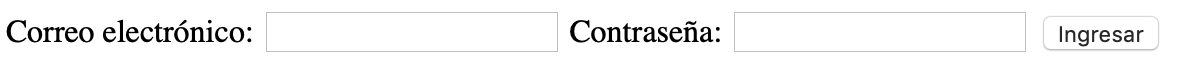
\includegraphics[scale=0.7]{anexos/html/imagenes/form_sample_login.png}

Note el uso de la etiqueta ``<label>''. Esta se utiliza para englobar a los
elementos ``<input>'', permitiendo mostrar un texto asociado a los mismos
que el visitante verá en el sitio, dandole indicaciones sobre qué es lo que
se espera que ingrese. Pueden usarse en su lugar párrafos de texto simple,
pero ``<label>'' brinda una ventaja adicional de usabilidad, cuando el
usuario da clic sobre el texto, el ``<input>'' se selecciona, y el usuario
ya puede comenzar a escribir, esto no ocurre con un párrafo. En particular
es una característica muy útil cuando se trabaja con elementos de tipo
``radio'' o ``checkbox''.

Las etiquetas ``<input>'' son muy útiles, pero en ocaciones no son suficientes.
Si se desea por ejemplo, que el usuario ingrese texto muy largo, se debe recurrir
a la etiqueta ``<textarea>''. Esta etiqueta presenta un cuadro de texto de
múltiples líneas, el cual se agranda automáticamente a medida que el usuario
escribe. Al igual que los ``<input>'', espera un atributo ``name'' para poder
ser procesado, pero no lleva ``type''.

También puede que se desee elegir de una serie de opciones de una lista, algo
que se logra con la etiqueta ``<select>'' (también espera un ``name'' como
atributo), la cual lleva dentro una o más etiquetas ``<option>''. Esta etiqueta
muestra una lista desplegable, en donde el usuario puede seleccionar una de las
opciones (dadas cada una por un ``<option>'' distinto).

A continuación hay un formulario que muestra el uso de etiquetas ``<textarea>'' y
``<select>''. También presenta un ``checkbox'' y un ``radio'' El formulario
permite al usuario ingresar un reclamo en el sitio
de una empresa proveedora de internet.

\begin{lstlisting}[language=XHTML]
<form action="servidor/procesar_ingreso" method="POST">
  <div>
    <label for="nombre">Su nombre:</label>
    <input type="text" name="nombre" id="nombre">
  </div>

  <div>
    <label for="motivo">Motivo del reclamo:</label>
    <select name="motivo" id="motivo">
      <option>No tengo conexión a internet</option>
      <option>Mi conexión anda lenta</option>
      <option>Mi conexión es intermitente</option>
      <option>Otro tipo de reclamo</option>
    </select>
  </div>

  <div>
    <label for="problema">Cuéntenos más sobre el problema:</label>
    <textarea name="problema" id="problema"></textarea>
  </div>

  <div>
    <input type="checkbox" name="reclamos_previos" id="reclamos_previos">
    <label for="reclamos_previos">¿Ya ha realizado reclamos en el pasado?</label>
  </div>

  <p>¿Desea que nos comuniquemos con usted?</p>
  <div>
    <input type="radio" name="comunicacion" id="comunicacion1">
    <label for="comunicacion1"></label>Comunicarse por correo electrónico</label>
  </div>  
  <div>
    <input type="radio" name="comunicacion" id="comunicacion2">
    <label for="comunicacion2"></label>Comunicarse por teléfono</label>
  </div>
  <div>
    <input type="radio" name="comunicacion" id="comunicacion3">
    <label for="comunicacion3">No comunicarse</label>
  </div>
  
  <div>
    <button type="submit">
      Enviar Reclamo
    </button>
    <button type="reset">
      Limpiar el formulario
    </button>
  </div>
</form>
\end{lstlisting}

Note como en este ejemplo las etiquetas ``<label>'' no envuelven al campo
que denotan, sino que se usa otra técnica, la cuál consiste en utilizar
un atributo ``for'' en ``<label>'' cuyo valor coincide con el valor del
atributo ``id'' del ``<input>'' que se encuentra marcando.

También se envuelve cada conjunto de ``<label>'' y ``<input>'' en una
etiqueta ``<div>'' que los agrupa semánticamente. Esto también logra el
efecto de mostrar un elemento debajo de otro en el formulario, ya que por
defecto, los ``<div>'' se muestran uno bajo el otro, mientras que los
``<label>'' y ``<input>'' se muestran todos en el mismo renglón.

El formulario anterior se vería algo así:

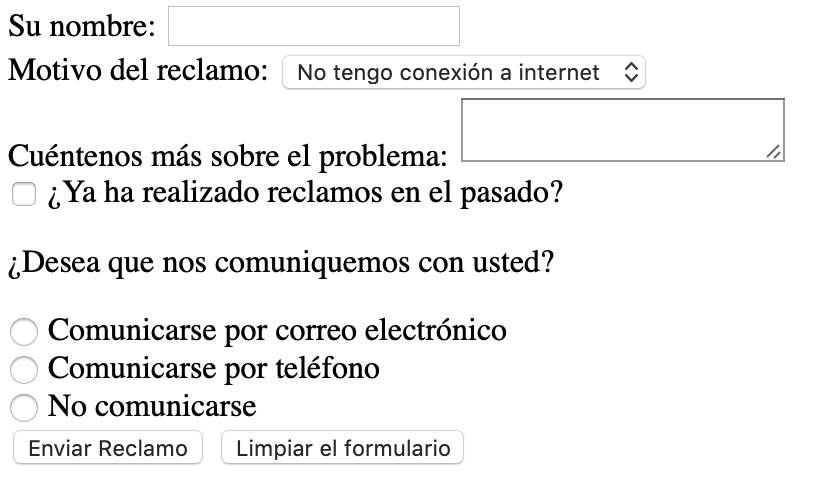
\includegraphics[scale=0.7]{anexos/html/imagenes/form_sample_no_css.png}

Los formularios pueden embellecerse con CSS. Existen incluso conjuntos de código
pre-hechos por terceros que uno puede utilizar para embellecer sus formularios
(y sus sitios en general). Estos códigos se agrupan en lo que se llama ``biblioteca'.
Con un poco de CSS el formulario anterior puede verse de la siguiente forma:

\centerline{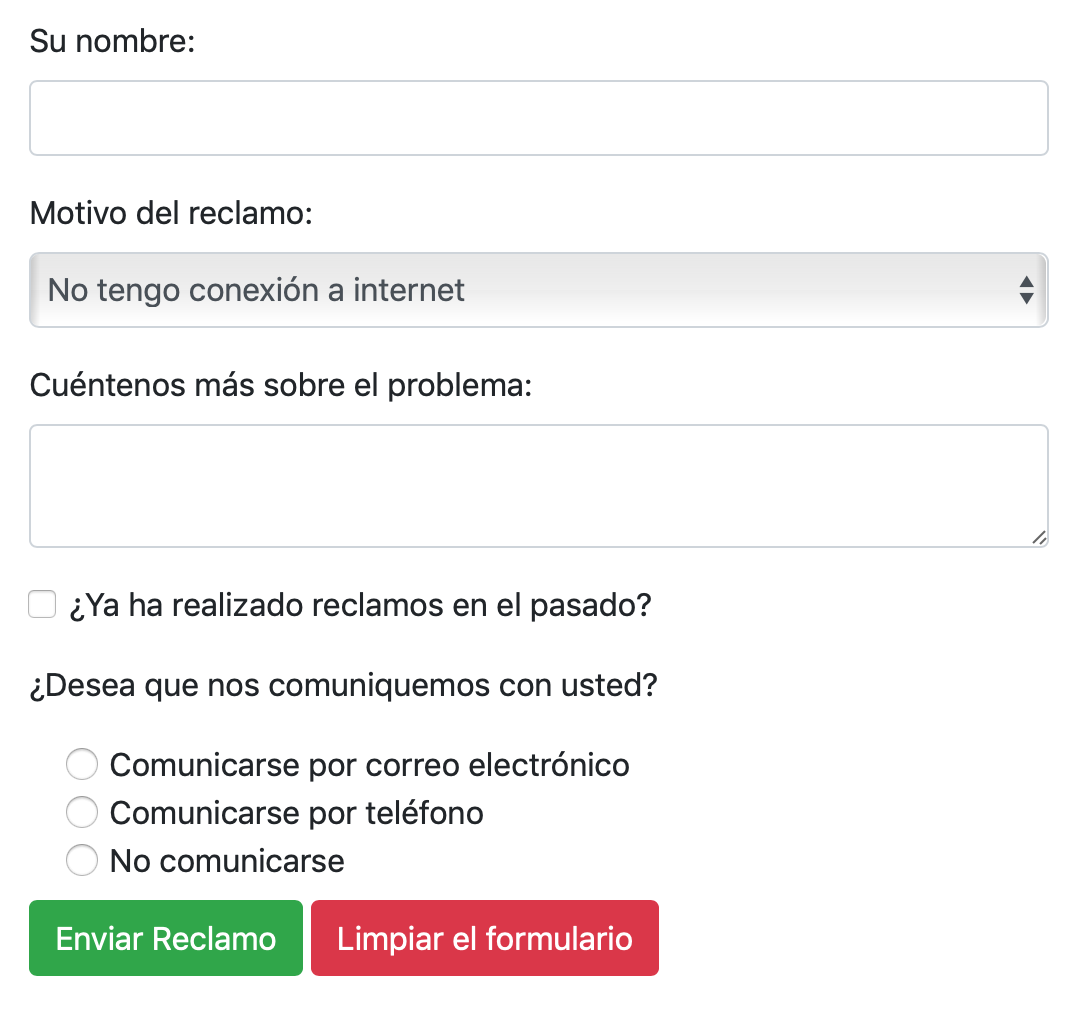
\includegraphics[scale=0.5]{anexos/html/imagenes/form_sample_css.png}}

Existen también otros atributos y particularidades que hacen a los formularios,
así como al procesamiento de los mismos. Estos detalles no son parte del presente,
y se recomienda al lector retomar estos temas cuando posea un conocimiento más
amplio de programación y de redes de computadoras.

\section{Actividades}

Los siguientes ejercicios se realizar de forma continuada, es decir, para
realizar el ejercicio 2 deberá realizar el ejercicio 1 previamente. Recomendamos
hacerlos en orden y no saltearse ninguno.

\begin{exercise}
Cree un documento HTML un sitio web que actuará como portal de noticias.
Recuerde de que el documento debe tener todas las partes protocolares
necesarias. Luego agregue los siguientes elementos a su sitio:
\begin{enumerate}[a)]
  \item Un título principal con el texto ``Últimas Noticias''.
  \item Una primer sección bajo el título ``Noticias deportivas''.
  \item Una segunda sección bajo el título ``Noticias del espectáculo''.
  \item Un párrafo descriptivo en cada sección indicando el tipo de noticias que
    el lector podrá encontrar.
\end{enumerate}

El resultado debería verse algo como:

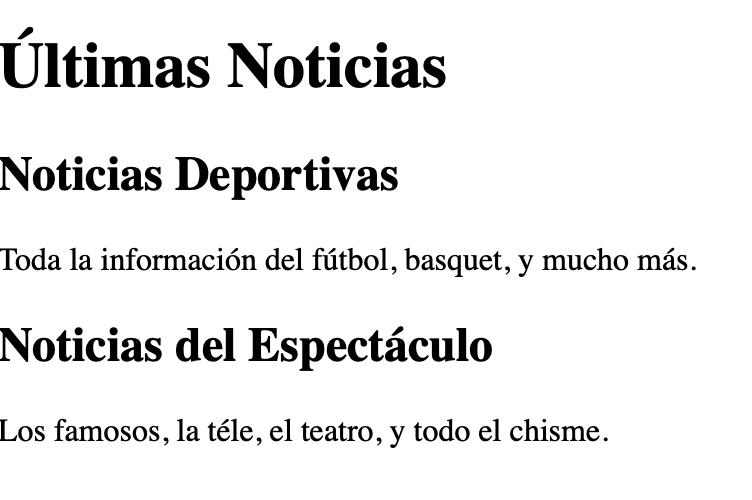
\includegraphics[scale=0.5]{anexos/html/imagenes/diario_1.png}
\end{exercise}

\begin{exercise}
Agregue dos artículos de noticias a cada sección del sitio anterior.
Puede buscar noticias en un medio de su preferencia, o inventarlas. Cada
noticia debe contar con un título (de menor jerarquía que los de las
secciones), y un copete (resumen de la noticia) en donde aparezcan algunas 
palabras o frases clave con énfasis. El resultado debería ser similar al
siguiente:

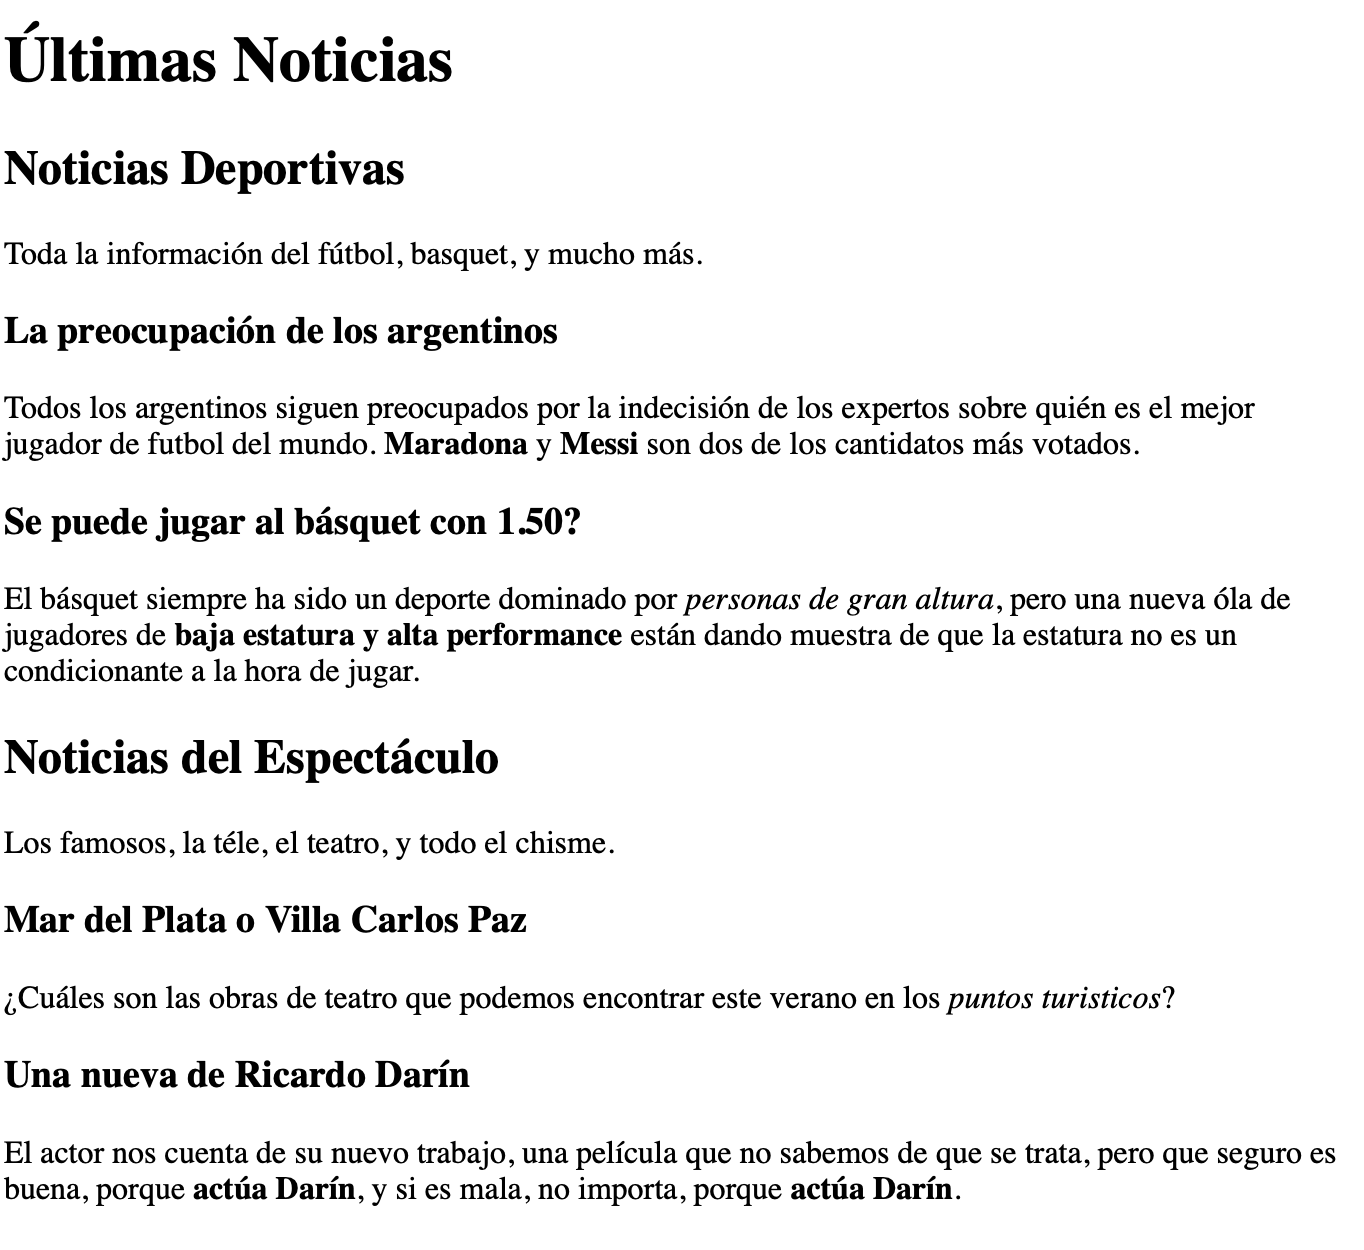
\includegraphics[scale=0.5]{anexos/html/imagenes/diario_2.png}
\end{exercise}

\begin{exercise}
Añada el link de referencia a los sitios de donde tomo las noticias
(o coloque un enlace a sitios de su preferencia si las inventó). Los
enlaces deben leerse con el texto ``Leer más''. El resultado debería
ser similar a este:

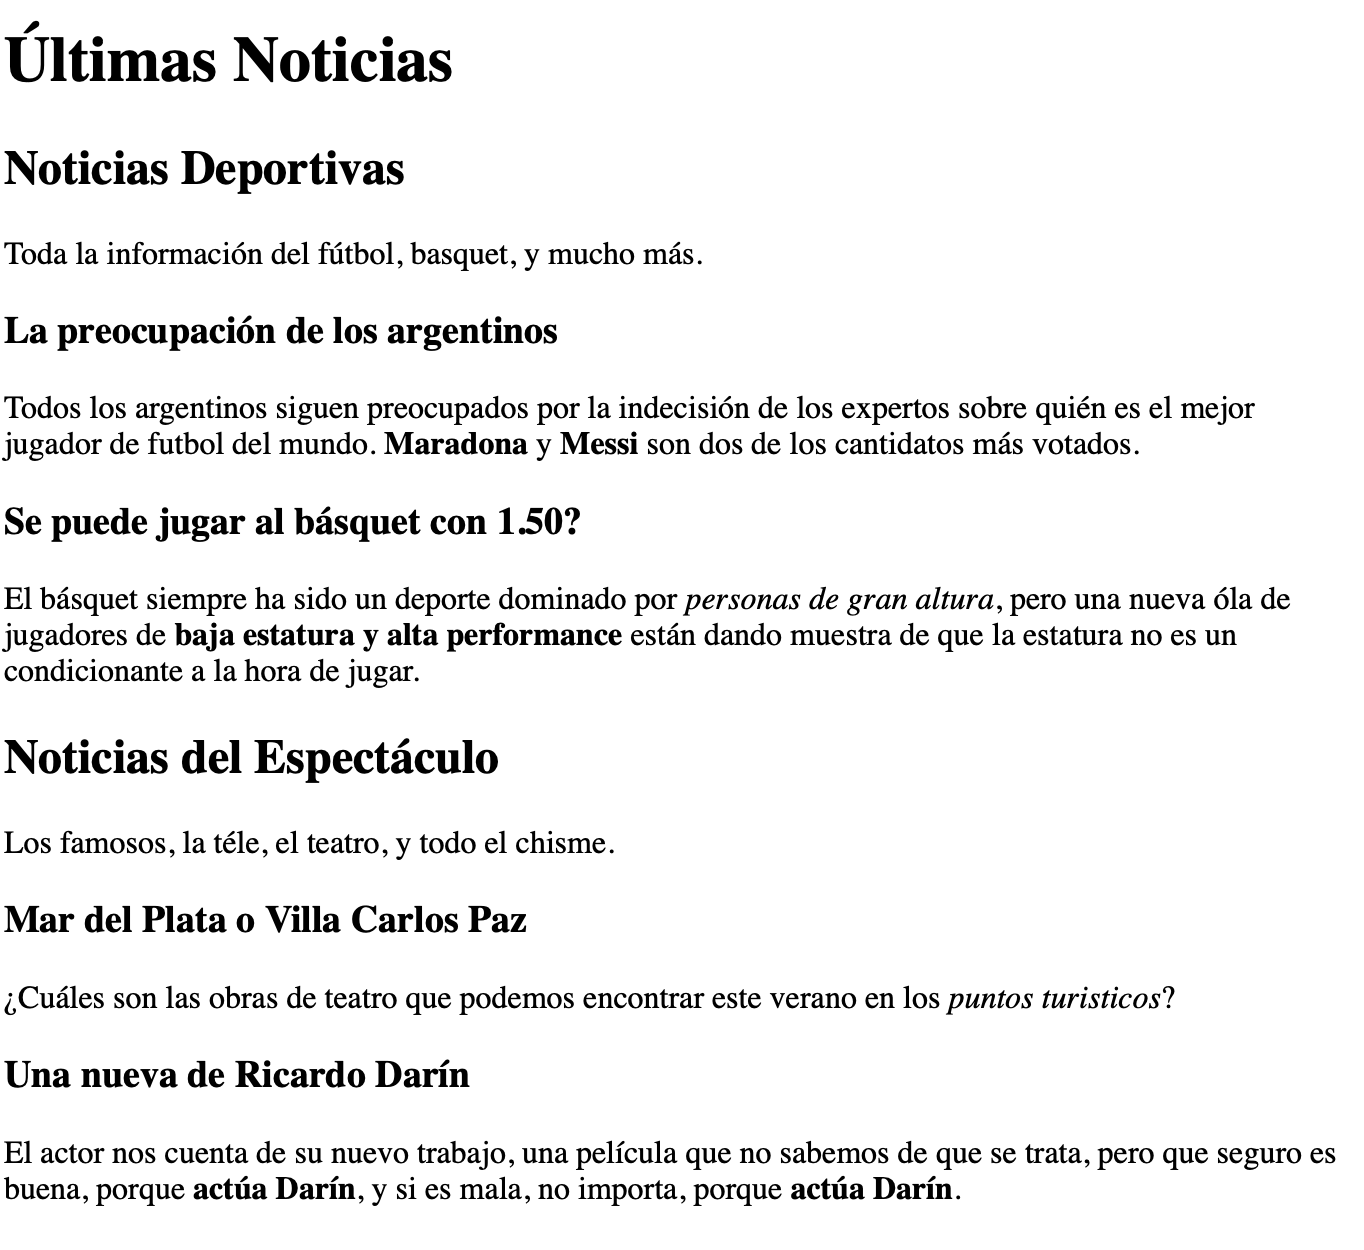
\includegraphics[scale=0.5]{anexos/html/imagenes/diario_3.png}
\end{exercise}

\begin{exercise}
Sume ahora, antes del título del diario, en una cabecera, una imagen que
actúe de logo del sitio. Puede tomar de internet una imagen que guste
como logo. Incluya también un pie de página con la información de copyright
del sitio. La misma debe contener el nombre del autor y el año en que
realizó el sitio. Tenga en cuenta que lo que antes eran posiblemente
simples secciones deberían ser ahora el contenido principal del sitio.
\end{exercise}

\begin{exercise}
Si realizó los ejercicios hasta ahora correctamente (es decir, ha colocado
todas las etiquetas de estructura semánticas que corresponde) debería ser
posible que su sitio luzca como la siguiente imagen:

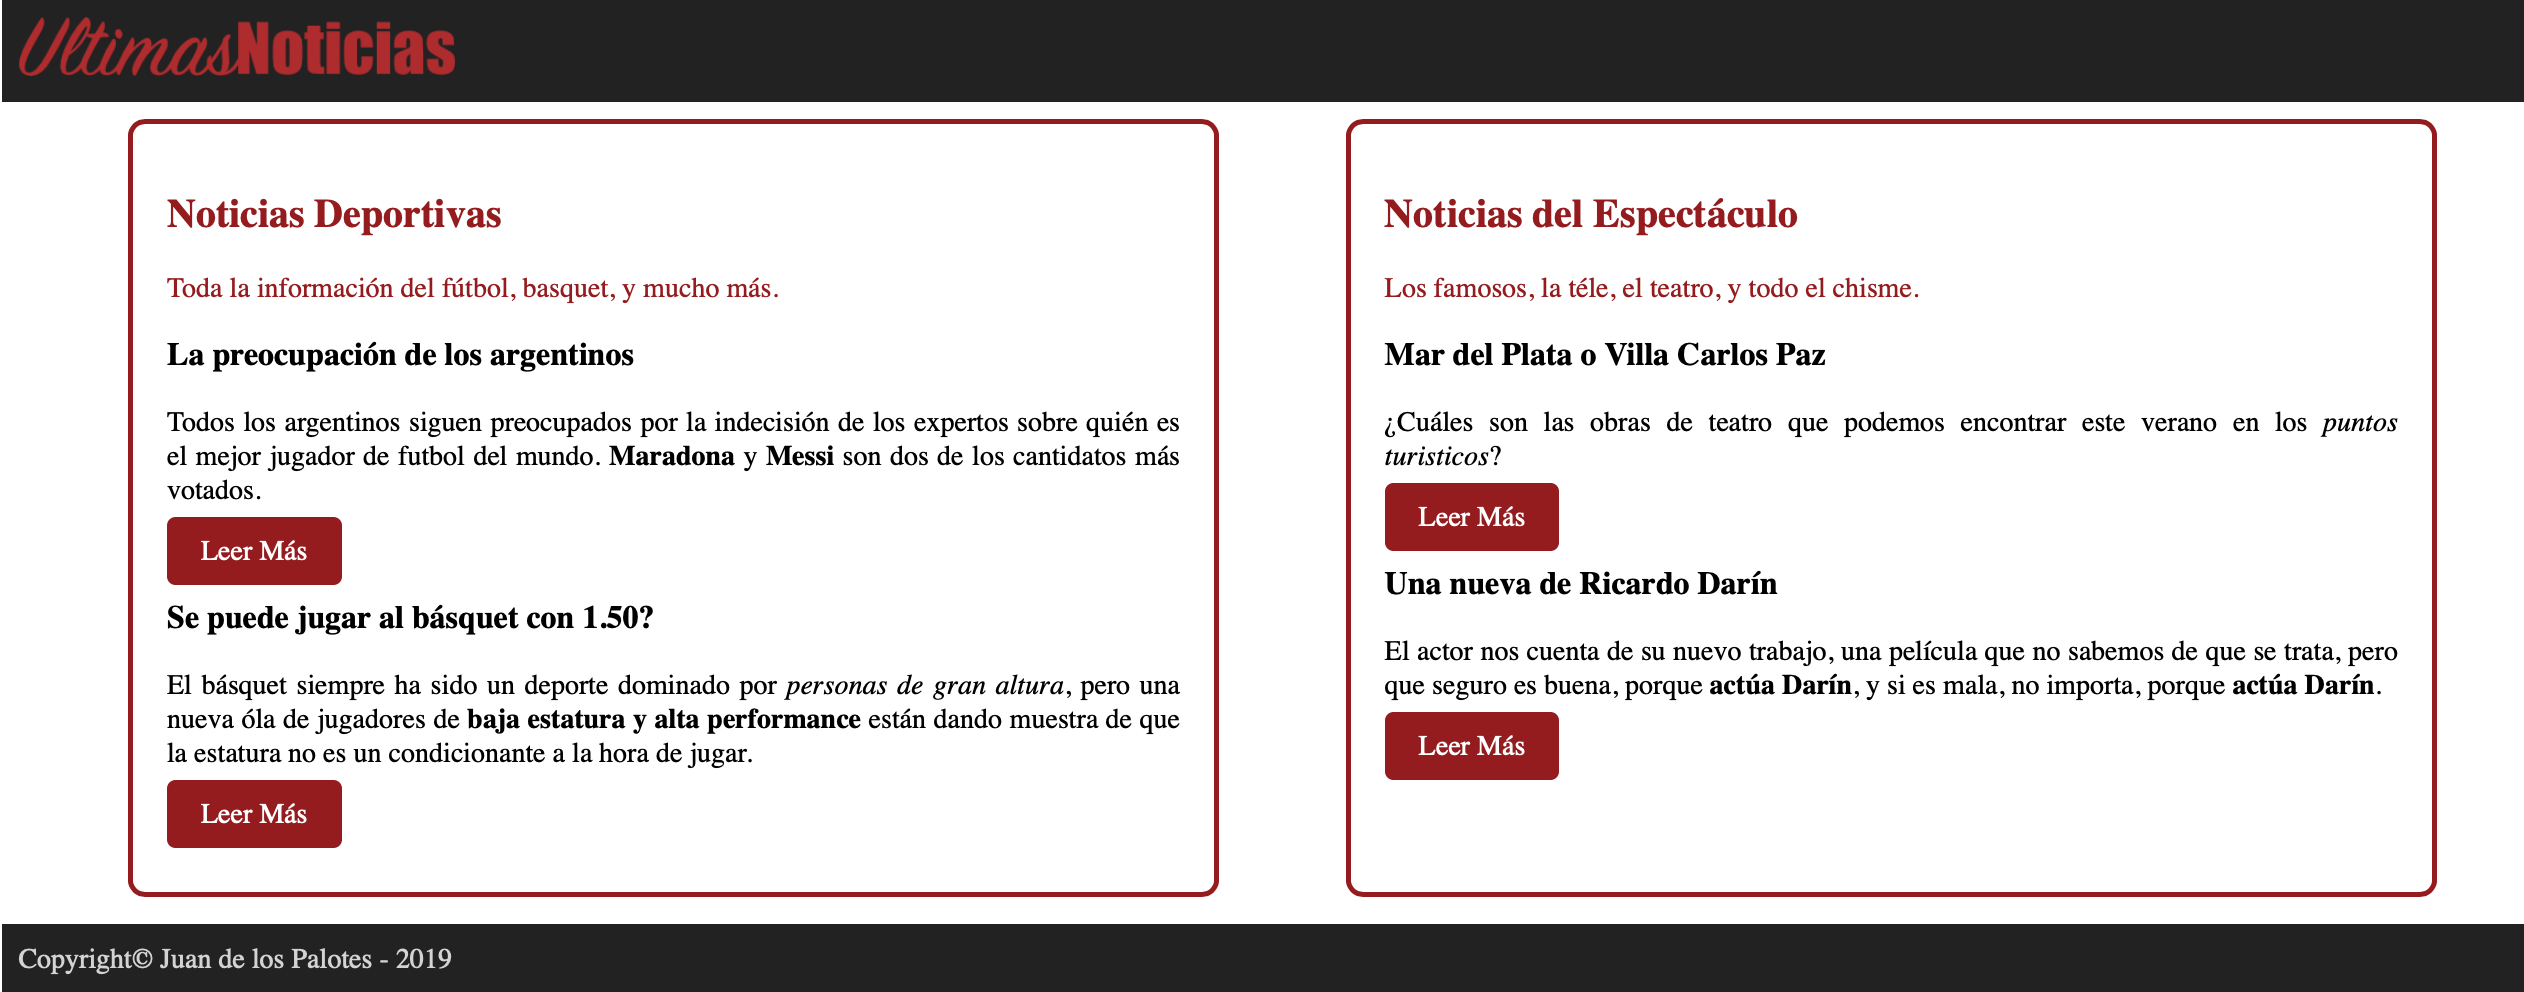
\includegraphics[scale=0.3]{anexos/html/imagenes/diario_4.png}

Para ello necesitaremos agregar en el ``<head>'' del sitio la siguiente
definición de CSS dentro de una etiqueta ``<style>'':

\begin{adjustwidth}{25pt}{10pt}
  \begin{lstlisting}[language=CSS]
header, footer {
  background-color: #222;
  color: lightgray;
}
footer {
  height: 40px;
}
header {
  height: 85px;
}
header, footer p {
  padding: 10px;
}
header h1, header h2, header h3,
header h4, header h5, header h6 {
  display: none;
}
header img {
  height: 35px;
  width: auto;
}
header nav {
  width: 100%;
  background-color: #222;
  margin-bottom: 20px;
}
header li {
  display: inline-block;
  padding: 10px;
}
header li%(*:*)hover {
  background-color: #555;
  cursor: pointer;
}
header a {
  color: white;
  text-decoration: none;
}
main {
  margin-top: 10px;
  display: flex;
  flex-direction: row;
}
section {
  justify-content: space-between;
  width: 40%;
  margin-left: 5%;
  border: 3px solid rgb(150, 25, 25);
  border-radius: 10px;
  padding: 20px;
}
section>h1, section>h2, section>h3,
section>h4, section>h5, section>h6,
section>p {
  color: rgb(150, 25, 25);
}
article p {
  text-align: justify;
}
article a {
  padding: 10px 20px;
  background-color: rgb(150, 25, 25);
  border-radius: 5px;
  color: white;
  text-decoration: none;
}
article a%(*:*)hover {
  background-color: rgb(200, 25, 25);
  text-decoration: none;
}
aside {
  text-align: center;
  background-color: cornflowerblue;
  color: darkred;
  width: 50%;
  margin: 0 auto;
  font-weight: bolder;
}
aside h1, aside h2, aside h3, aside h4,
aside h5, aside h6 {
  animation: blinker 2s linear infinite;
}
@keyframes blinker {
  50% { opacity: 0; }
}
  \end{lstlisting}
\end{adjustwidth}
\end{exercise}

\begin{exercise}
Agregue en la cabecera una barra de navegación, que contenga una lista
no ordenada de enlaces a las secciones del sitio. Las mismas son:
Política, Policiales, Deportes y Espectáculos.
El resultado debe ser como el siguiente:

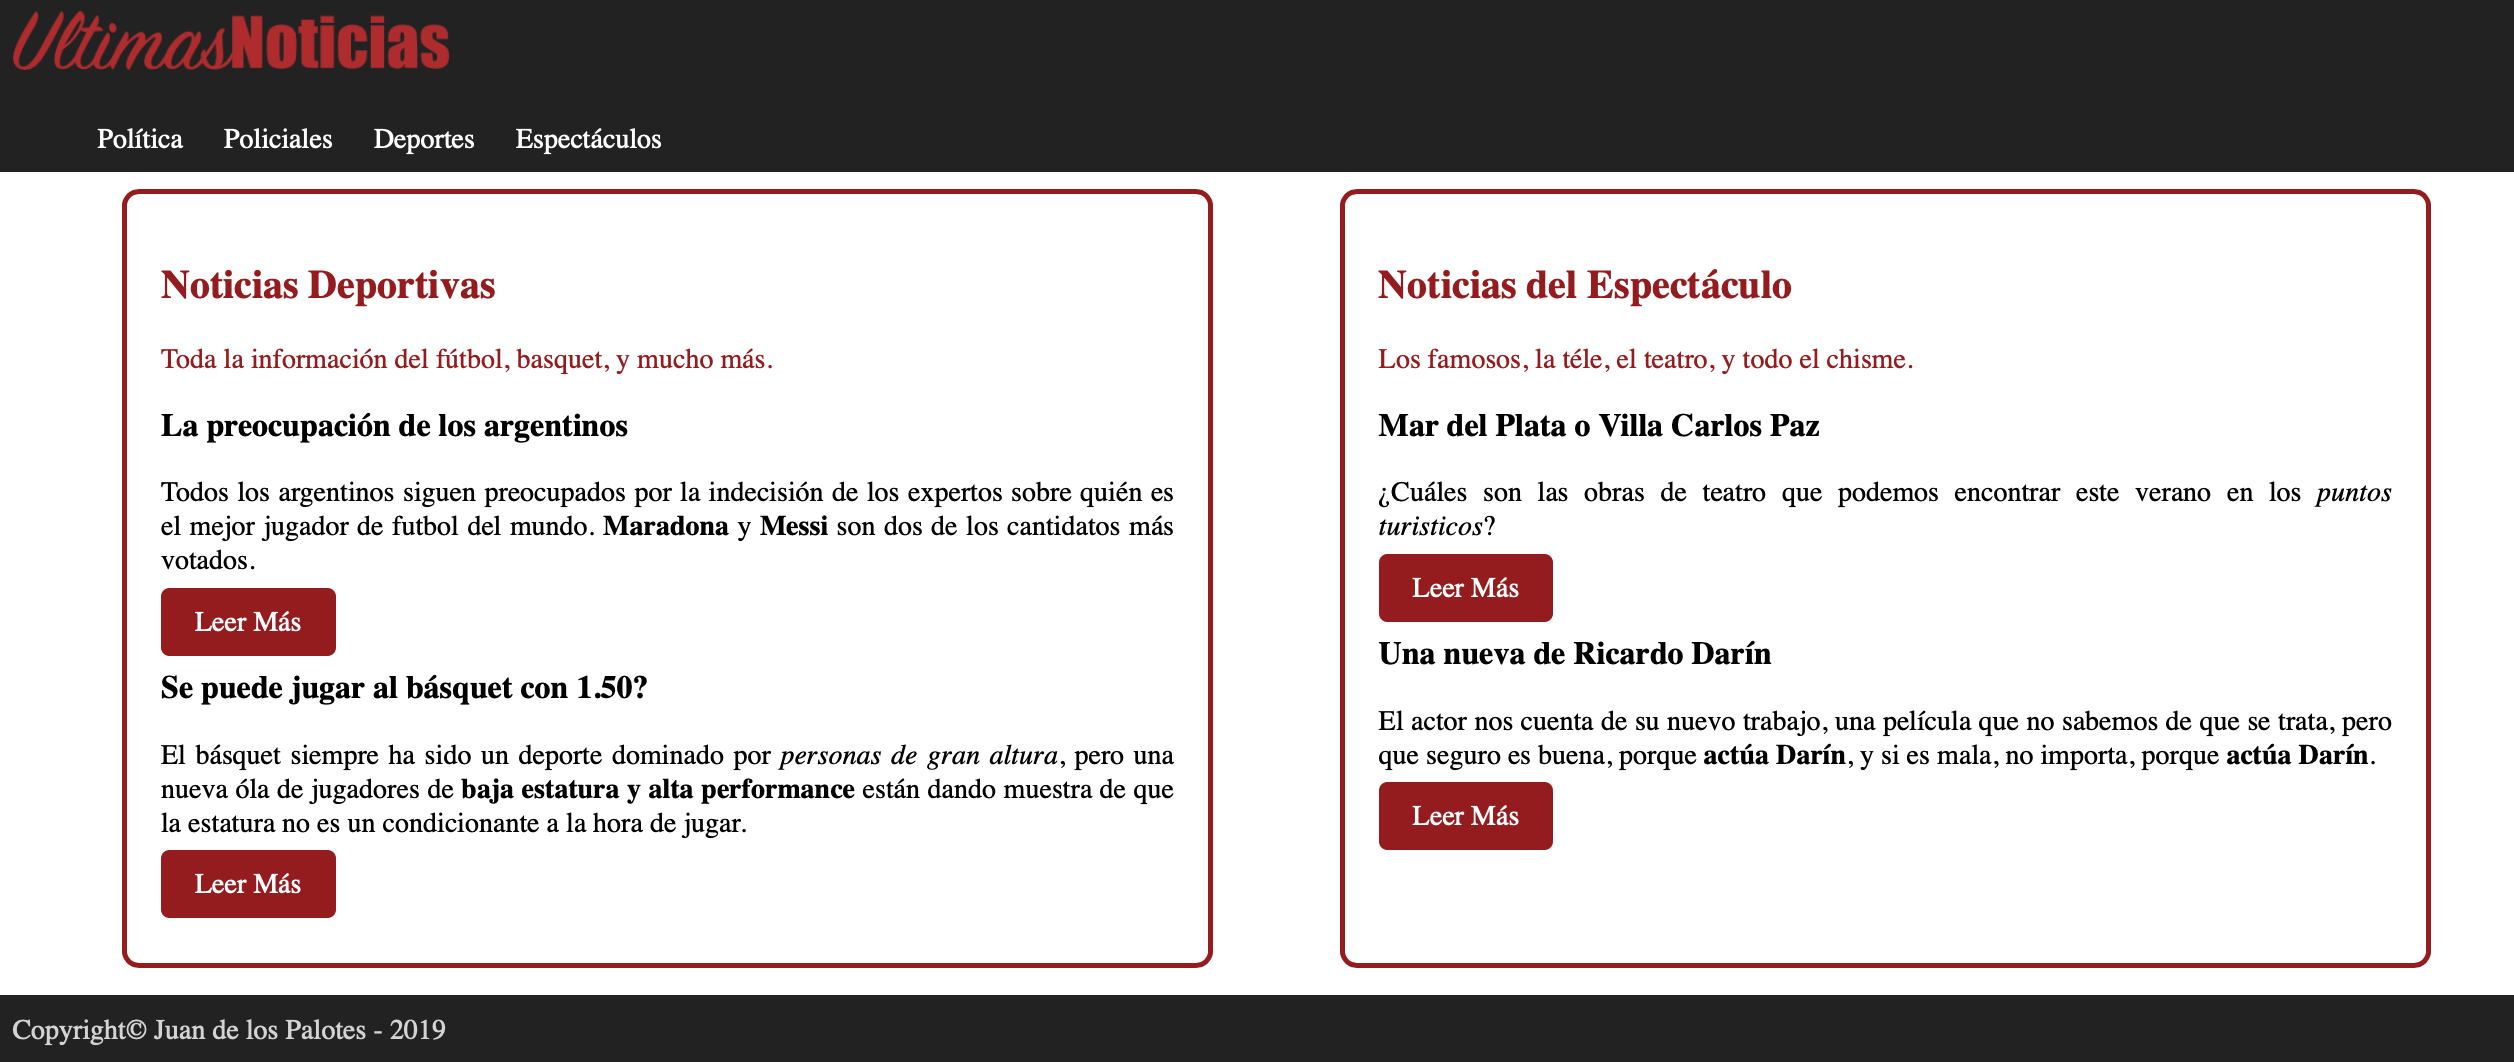
\includegraphics[scale=0.3]{anexos/html/imagenes/diario_5.png}
\end{exercise}

\begin{exercise}
Agregue justo sobre el pie de página una publicidad. Coloque en ella
un título o dos títulos de nivel dos en adelante, y un párrafo de
texto. El resultado se verá algo así:

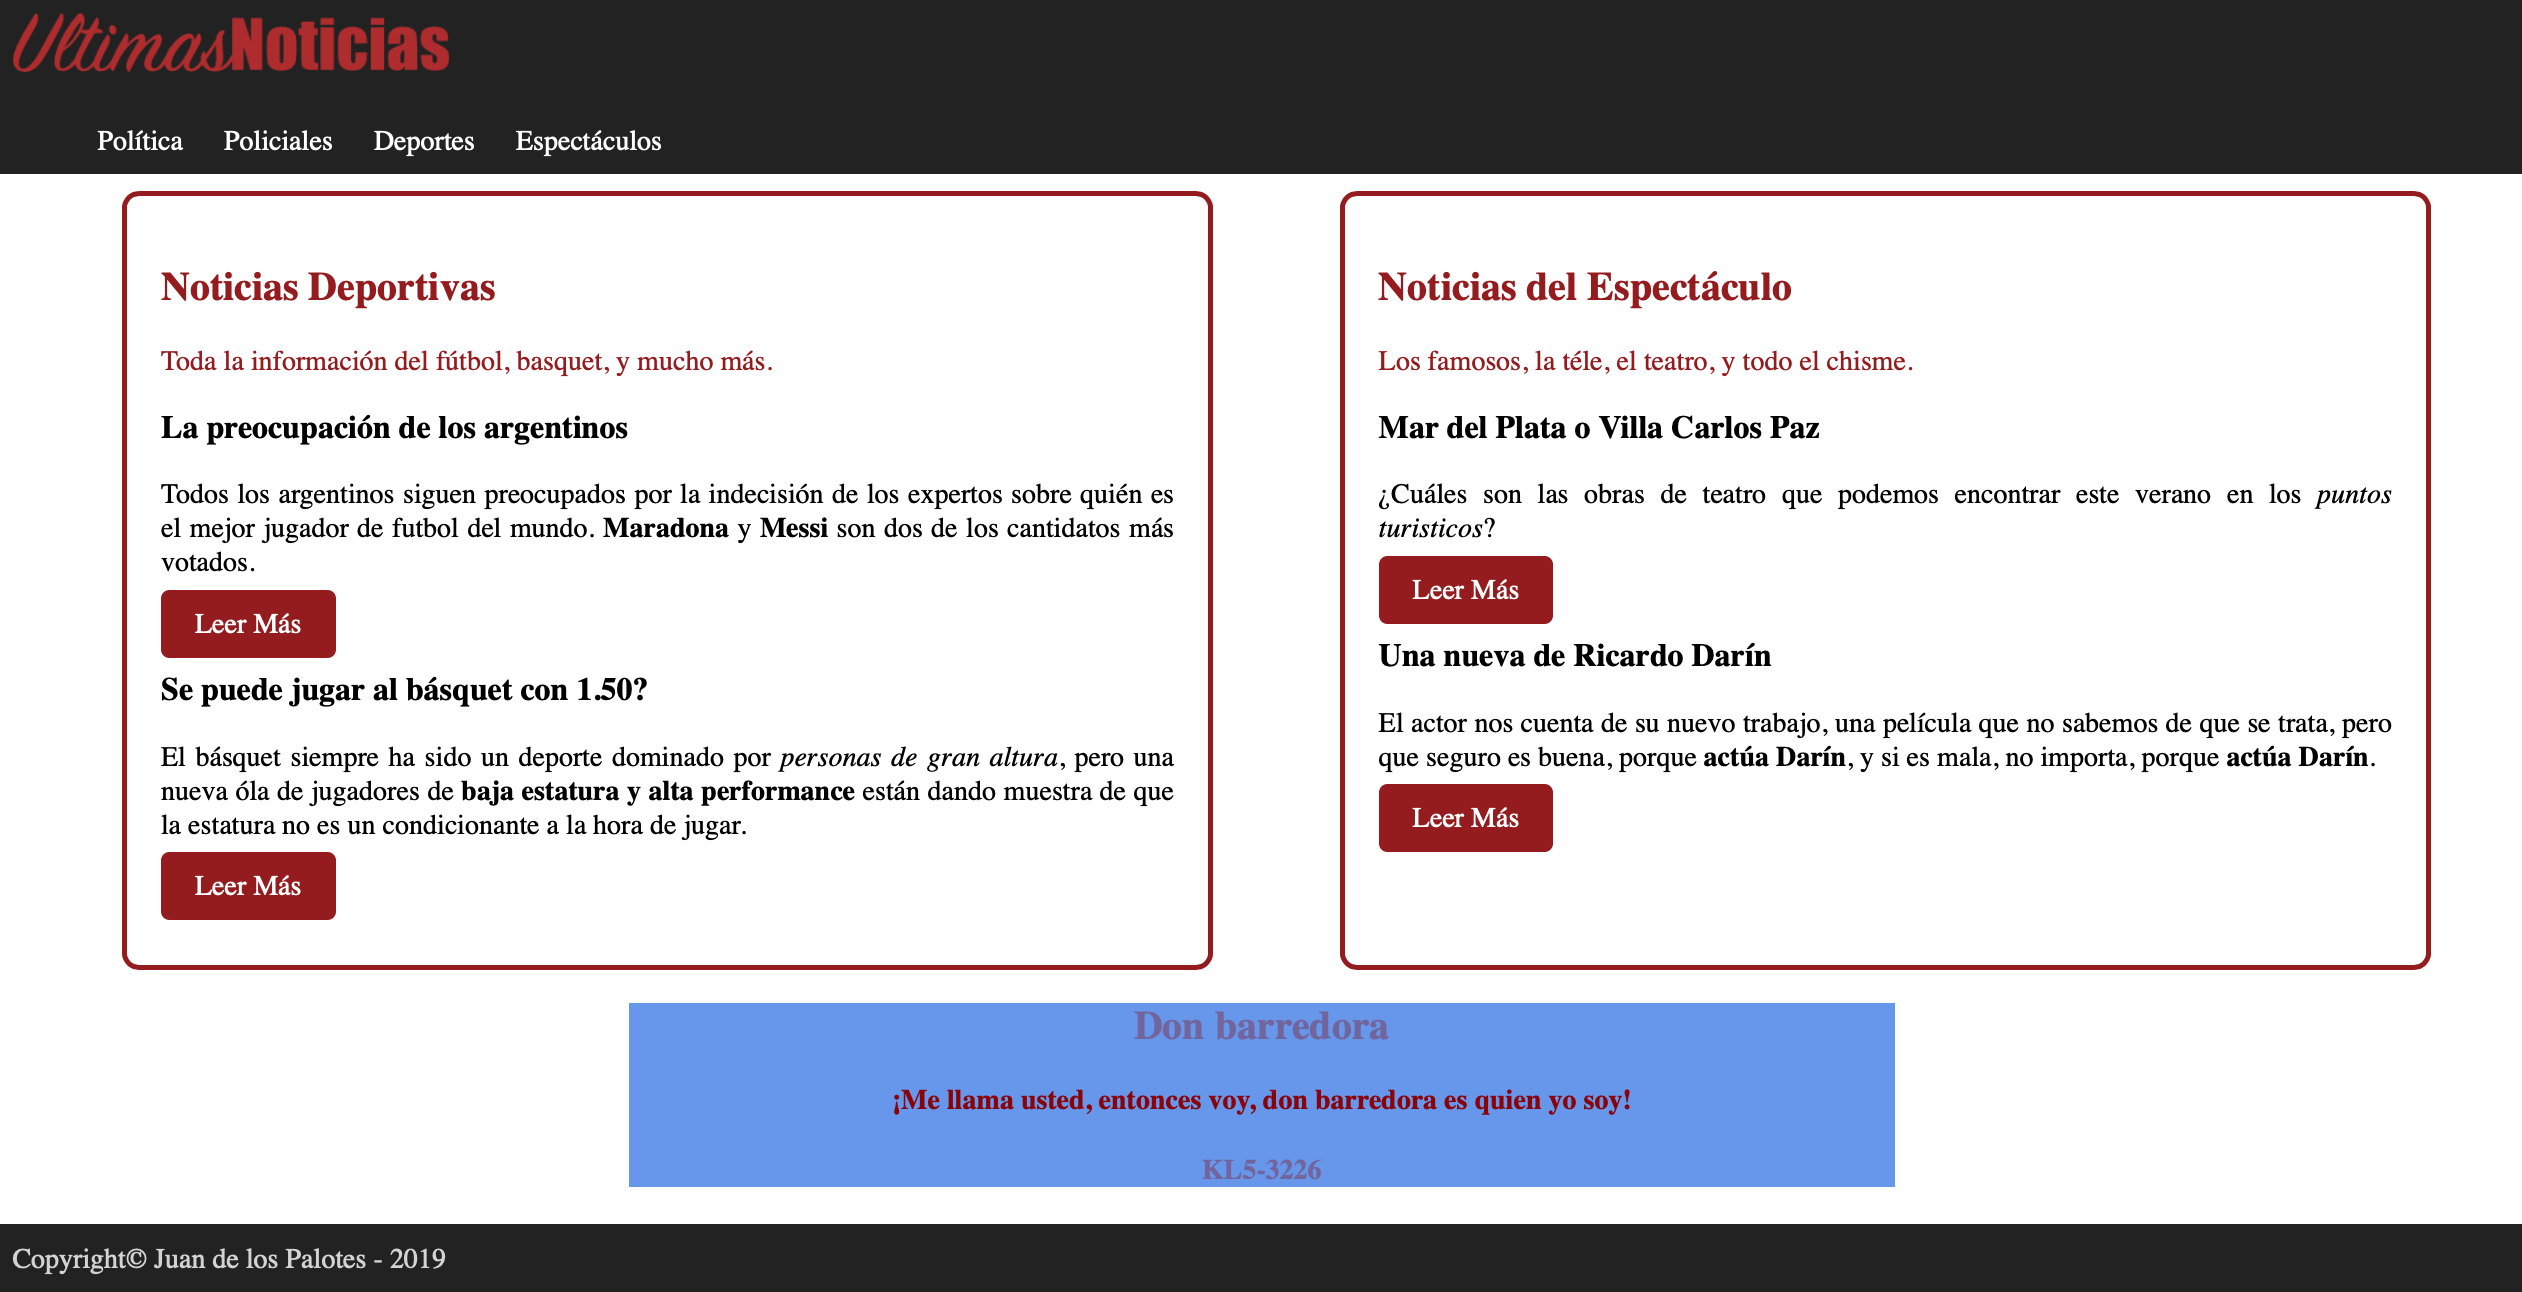
\includegraphics[scale=0.3]{anexos/html/imagenes/diario_6.png}
\end{exercise}

\begin{exercise}
  Valide el código que ha generado con el validador oficial de la W3C.
  Si el código pasa exitosamente las pruebas, significa que el código
  no viola los estándares (aunque no significa que siga buenas prácticas
  de estilo, por lo que no necesariamente es un buen código).

  De encontrarse con errores al momento de validar, corrija su código
  hasta que este sea válido. Puede encontrar el validador en:

  \href{https://validator.w3.org/nu/\#file}{https://validator.w3.org/nu/\#file}
\end{exercise}

\begin{exercise}
Se pide que diseñe una página web que contenga un formulario web capaz de
cargar ordenes médicas para pacientes que requieren reposo laboral. El 
formulario debe contener los siguientes campos:
\begin{itemize}
  \item Un campo de texto para el nombre del médico que firma la orden.
  \item Un campo de texto para el número de matricula del médico que firma la orden.
  \item Un campo de selección radial que permita elegir si el número de
    matricula corresponde a la matricula nacional o provincial.
  \item Un campo de texto para el nombre del paciente.
  \item Un campo de selección que permita elegir la cantidad de horas de reposo.
    Deben haber 4 opciones: ``24 horas'', ``48 horas'', ``72 horas'', ``hasta alta médica''.
  \item Un campo de selección (checkbox) que se pueda marcar si el paciente
    tiene obra social, y desmarcar en caso negativo.
  \item Labels para cada uno de los campos.
  \item Un botón para enviar el formulario.
\end{itemize}
El formulario deberá utilizar el método GET, y su acción deberá indicar como
valor ``\#'' (solo el signo numeral).

Puede utilizar el siguiente código CSS:
\begin{adjustwidth}{25pt}{10pt}
  \begin{lstlisting}[language=CSS]
label {
  display: block;
  margin: 5px 0;
}
  \end{lstlisting}
\end{adjustwidth}
Esto logrará que los elementos aparezcan como en la imagen a continuación:

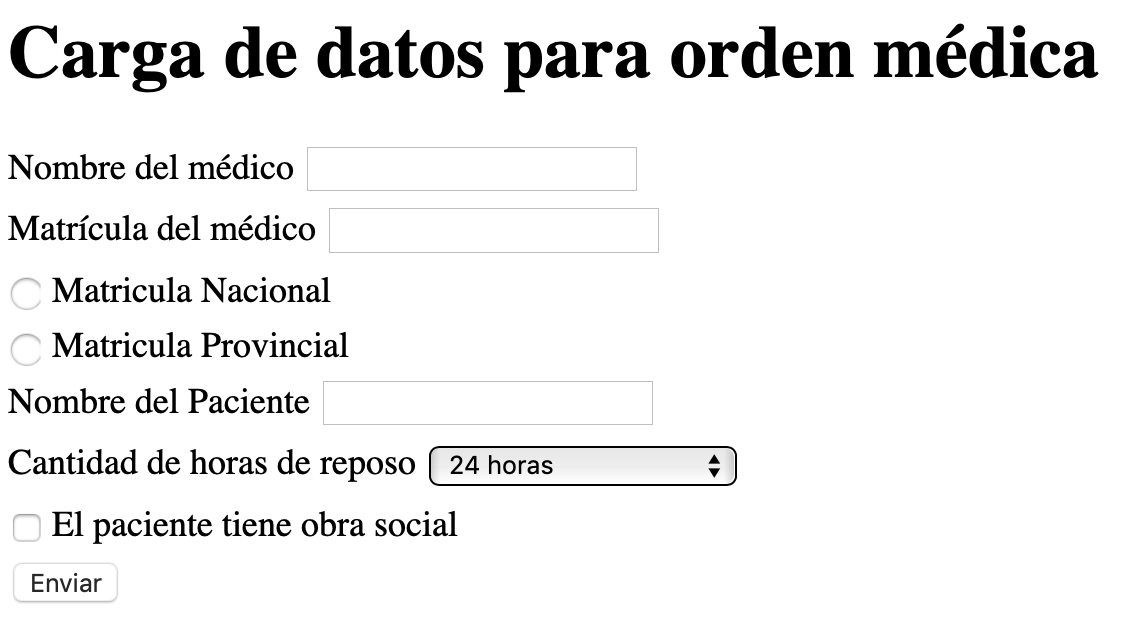
\includegraphics[scale=0.65]{anexos/html/imagenes/formulario_1.png}
\end{exercise}

\begin{exercise}
Diseñe una página web que contenga un título principal con el texto
``Mundiales de la FIFA'', y luego una tabla de doble entrada, donde las filas
corresponden cada una a un mundial distinto. Deben haber tres columnas, la primera
indicando en que lugar del mundo se realizó el evento, y la segunda y
tercer columna indicando el campeón y subcampeón respectivamente.
Incluya al menos los mundiales de los siguientes años:
\begin{itemize}
  \item 2002
  \item 2006
  \item 2010
  \item 2014
  \item 2018
\end{itemize}

Puede utilizar el siguiente código CSS para que la tabla quede más fácil
de visualizar:
\begin{adjustwidth}{25pt}{10pt}
  \begin{lstlisting}[language=CSS]
table {
  border: 3px solid rgb(150, 25, 25);
  border-collapse: collapse;
  border-spacing: 0;
}
table tr:nth-child(odd) {
  background-color: rgb(255, 175, 175);
}
table tr:nth-child(1) {
  background-color: rgb(150, 25, 25);
  color: white;
}
table td {
  padding: 3px 5px;
}
  \end{lstlisting}
\end{adjustwidth}
El resultado de la página debería ser el siguiente.

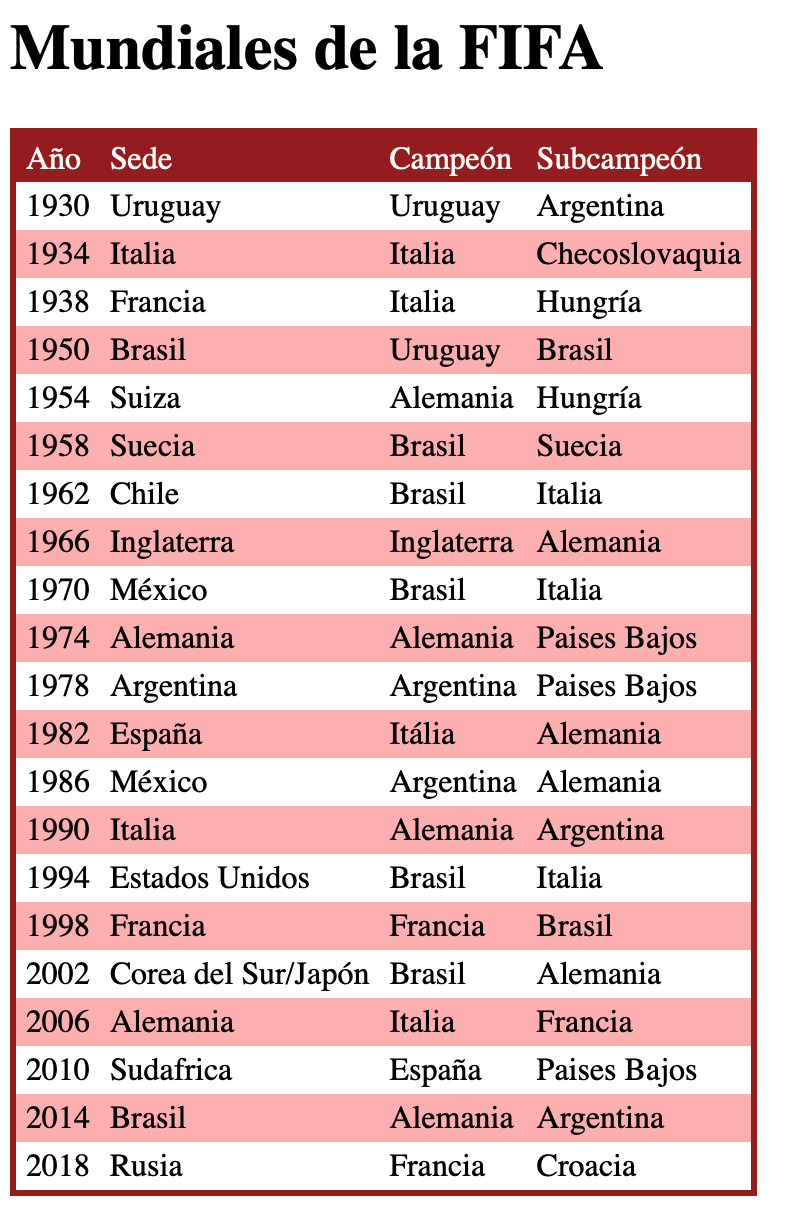
\includegraphics[scale=0.65]{anexos/html/imagenes/tabla.png}
\end{exercise}